\documentclass[]{Photos_interface_design}
\usepackage{graphicx}
\usepackage{hyperref}
\usepackage{eurosym}
\usepackage{pifont}
%\usepackage{tocloft}
\usepackage{amsmath}
\usepackage{subfigure}
\usepackage{booktabs}

\makeatletter
\renewcommand*\l@subsection{\@dottedtocline{2}{1.5em}{2.0em}}
\renewcommand*\l@subsubsection{\@dottedtocline{3}{3.0em}{3.0em}}
\makeatother

\begin{document}

\maketitle

\tableofcontents\pdfbookmark[0]{Table of Contents}{toc}

\newpage

\section{Introduction}
For a long time, {\tt PHOTOS} Monte Carlo \cite{Barberio:1990ms,Barberio:1993qi} 
has been used for the generation of bremsstrahlung in the decay of particles and resonances.
Over the years the program has acquired
popularity and it evolved into a high 
precision tool \cite{Golonka:2006tw}. Since version 2.15 of the program become 
public in the year 2005 and multi-photon radiation was 
introduced \cite{Golonka:2005pn}, there were no further public upgrades 
of the program. However the effort on documentation and tests was going on;
 phase space treatment was shown to be 
exact \cite{Nanava:2006vv} and for several 
processes \cite{Golonka:2006tw,Nanava:2006vv,Nanava:2009vg}
an exact matrix element was studied with the help of optional weights.
Benchmark distributions, including comparisons with  
other simulation programs, were collected on the program web page \cite{Photos_tests}. 

 Such high precision applications require good control of the event record content on which {\tt PHOTOS} operates. On one side it 
requests skills and experience of the user and on the other it provides 
the flexibility necessary for the study of effects like, for example, systematic errors for 
measurements of anomalous couplings or W cross section. Methods of 
correlated samples  can be applied\footnote{To exploit such methods in 
the high precision regime, good control of matrix element properties is necessary.
As was shown in \cite{Kleiss:1990jv}, complications for such methods arise at the second order matrix element only, thus at the precision level of 
$(\frac{\alpha_{QED}}{\pi})^2 \simeq 10^{-5}$.}. 

Until recently {\tt HEPEVT} \cite{Altarelli:1989wu} was used as the structure for 
communication between physics Monte Carlo programs and detector/reconstruction 
packages. Experimental physicists used {\tt HEPEVT} 
for their own applications  as well. Recently, to gain  flexibility, {\tt FORTRAN} is being replaced by C++ and 
instead of {\tt HEPEVT}, the C++ event structure called {\tt HepMC} \cite{Dobbs:2001ck}
is used. Nothing prevents 
moving {\tt PHOTOS} to an environment based on  {\tt HepMC}
and to rewriting the whole (beginning with the event record interface)
of {\tt PHOTOS}\footnote{An up-to-date version of the code described in this paper is
available from the web page of our project~\cite{photosC++}. 
  }
 to C++. In fact implementation of the algorithm in that language 
is clearer and easier to
 maintain. Because of its design the {\tt PHOTOS} algorithm benefits from the object 
oriented features of C++. It is our third program, after {\tt MC-TESTER} \cite{Davidson:2008ma}
and the {\tt TAUOLA} interface \cite{Davidson:2010rw}, previously ported to {\tt HepMC} and C++.
This completes the main step of migration of these three programs to the new style.

Such migration is convenient for the users too; they can now work
with  homogeneous C++ software. From the physics point of view, transformation 
of {\tt PHOTOS} 
from {\tt FORTRAN} to C++  brings some benefits as well.
The channel dependent, complete first order matrix elements of {\tt PHOTOS}, in {\tt FORTRAN},
 are available only 
in special
kinematical configurations. With the help of the new  event record interface they will become
available for general use.
For that purpose, better access to the information necessary to orient the spin state of decaying particles
is now provided.



Our paper is organized as follows. Section \ref{sec:requrements} is devoted
to a description of physics information which must be available in the event
record for the algorithm to function. Later, particular requirements for the 
information stored in {\tt HepMC} are given. Section \ref{sec:design} describes
the program structure. In Section \ref{sec:extensibility} methods prepared for 
future extensions to improve the physics precision of the generator are explained.
Section \ref{sec:tests} presents the program tests and benchmarks. 
A summary, section \ref{sec:summary}, closes the paper.
There are three appendices \ref{Interface to PHOTOS}, 
\ref{sec:User Guide} and \ref{sec:User Configuration} attached to the paper.
Respectively, they describe the interface to the old {\tt FORTRAN} part of the code,
provide a user guide and explain the program configuration methods and parameters. 


\section{Requirements of the {\tt PHOTOS} Interface}
\label{sec:requrements}
The algorithm of {\tt PHOTOS} Monte Carlo can be divided into two parts.
The first, internal part, operates on elementary decays. Thanks to carefully 
studied properties of the 
QED (scalar QED) algorithm, with certain probability, 
it replaces the kinematical configuration of the Born level decay with a new one, 
where a bremsstrahlung photon or photons
are added and other particle momenta are modified. This part of the program is sophisticated from the physics 
point of view \cite{Golonka:2006tw,Nanava:2006vv},
but from the point of view of data structures the algorithm is simple.
That is why the gain from re-writing this part of the program to C++ is rather
limited and will be postponed to a later step of the project development.
On the other hand, there are not many obstacles for such a transformation to be
performed. In fact it was already done
previously \cite{photosplus}, but the resulting program was developed too early 
and did not attract users because of a lack of a C++ event record format standard at that time.

The typical results of high energy process simulation are events of complex structure.
They include, for example, initial state parton showers, hard scattering parts,
hadronization and finally chains of cascade decays of resonances. 
A structure similar to a tree is created, but properties of such data structures
are sometimes violated.
For its action, {\tt PHOTOS} needs to scan an event record (tree) 
and localize branchings where
it is supposed to act. The decaying particle (mother) and its primary decay products
(daughters) have to be passed into the internal event structure of {\tt PHOTOS}. 
Finally for each daughter a list of all its subsequent decay products has to be 
formed. Kinematical modifications need to be performed on all descendants of the modified daughter.

In the new, C++ version of this part of the algorithm, additional functionality
is added.
The first mother of the decaying particle will be localized and passed together with  
the elementary branching to the internal part of the program. 
Prior to activation of the algorithm for  photon(s) generation and kinematic construction,
 the whole decay branching 
(supplemented with its mother(s))
will be boosted into the decaying particle's rest frame and the first mother
will be oriented along the $z$ axis. 
In many cases, the spin state of the decaying particle  can be calculated from kinematics of its production process.
Later it can be passed on to the code which calculates the matrix element for our branching.


At present, the part of the code responsible for photon(s) generation and kinematic 
construction is left in  {\tt FORTRAN}. It does not feature the options presented above yet.


Before an actual description of the program, let us list the tasks the event record interface must be able to perform:
\begin{enumerate}
\item a method to read  particles stored in the event tree.
\item a method to add or modify particles of the event tree.
\item a method to search for elementary decays over the entire tree of the event.
\item a method to form lists of all subsequent decay products originating from each elementary decay product.
\item a method to localize the first mother of the decaying particle. 
\item a method to localize the second mother for a special case of $t \bar t$ pair.
\end{enumerate}


\subsection{C++ and HepMC Specific Requirements}

The C++ version of the {\tt PHOTOS} interface implements all functionality
of its predecessor, the {\tt PHOTOS} version 2.15 \cite{Golonka:2005pn} coded in {\tt FORTRAN}.
The program is prepared for installation of the process-dependent correcting weights of refs 
\cite{Golonka:2006tw,Nanava:2009vg} into its public available version. 
{\tt PHOTOS} can be attached to any Monte-Carlo program,
provided that its output is available through a {\tt HepMC} \cite{Dobbs:2001ck} event record.
It seems that {\tt HepMC} will
remain a generally accepted standard for the near future. However,
already now several different options for how {\tt HepMC} is used are
widespread. The possibility of the flexible  adaptation of our event record 
interface to different
options has been considered in the design,  drawing experience
from {\tt MC-TESTER} \cite{Davidson:2008ma,Golonka:2002rz}.
We have also
envisaged the possibility that {\tt HepMC} may one day be replaced by another
standard of event record, and we have provided a way to extend
the interface to a possible new event record standard as well.

\subsection{Object Oriented Event Records  -- The Case of {\tt HepMC}}
% nd-the next paragraph repeats information that's already stated in other places.
% zbw: this is short intro to HepMC, later contexts of our use dominate. Nadia is it OK for you?
 In adapting the {\tt PHOTOS} interface to the C++ event record format
the difference between the {\tt HEPEVT} event record, used in the {\tt
  FORTRAN} version of the {\tt PHOTOS} interface, and the {\tt HepMC} event
record, which is used for the C++ based interface, has to be taken into
account.  In the first case 
a {\tt FORTRAN common block} containing a list of particles with their properties and
with integer variables denoting pointers to their origins and
descendants is used.  The {\tt HepMC} event structure is built from vertices,
each of them having pointers to their origins and descendants. Links
between vertices represent particles or fields.  Fortunately, in both {\tt
  FORTRAN} and C++ cases, the event is structured as a
tree\footnote{At least in principle, because in practice its
properties may be rather like a graph without universally defined
properties.  This makes our task challenging.}; the necessary
algorithms are analogous, but nonetheless different. The {\tt HepMC}
structure based on vertices is more convenient for the {\tt PHOTOS}
interface. 

In {\tt HepMC}, an event is represented by a {\tt GenEvent} object,
which contains information such as event id,
units used for dimensional quantities in the event and the list of produced particles. The particles
themselves are grouped into {\tt GenVertex} objects allowing access to mother
and daughter particles of a single decay. Vertices provide an easy way
to point to the whole branch in a decay tree that needs to be accessed,
modified or deleted if needed. The information of a particle  itself is stored
in a {\tt GenParticle} object containing the particle id, status and momentum
as well as information needed to locate its position in the decay tree.
This approach allows traversing the event record structure in several different
ways.

The {\tt HepMC} event record format is  evolving with time, making it necessary
 to adapt
the code to new versions. The
{\tt HepMC} versions 2.06, 2.05  and 2.03 were used  in the final tests of our 
distribution. 

Evolution of the {\tt HepMC} format itself is not a crucial problem.
In contrast, conventions on how physics information is  filled into {\tt HepMC}
represent the main source of technical and also physics 
challenges for our interface. 
This is quite similar to the previous
{\tt HEPEVT - FORTRAN} case. Let us discuss this point in more detail now.

\subsubsection{Event Record Structure Scenarios}



While many Monte-Carlo generators (e.g. {\tt PYTHIA 8.1} \cite{Sjostrand:2007gs}, 
HERWIG++ \cite{Bahr:2008pv}), SHERPA \cite{Gleisberg:2008ta} can 
store events in {\tt HepMC} format, the  representations of
these events are not subject to strict standards,  which can therefore
vary between Monte-Carlo generators or even physics processes. Some examples
of these variations include the conventions of status codes, the  way
documentary information on the event is added, the direction of pointers at a vertex
and the conservation (or lack of conservation) of energy-momentum at a vertex.
Below is a list of properties for basic scenario we have observed in Monte-Carlo
generators used for testing the code.

This list will serve as a declaration for convention of  {\tt HepMC} filling, which  the 
interface should  be able to interpret correctly.

\begin{itemize}
  \item \textbf{4-momentum conservation} is assumed for all vertices in the event record where {\tt PHOTOS} is expected to act.
  \item \textbf{Status codes:} only information on whether a given particle is incoming, outgoing or intermediate will be used. We assume the codes used will be 0, 1 or 2 like in HEPEVT. All other codes will be treated as
equivalent to  the status 2.
  \item \textbf{Pointers at a vertex} are assumed to be bi-directional. That is, it is possible to traverse the record structure from mother to daughter and from daughter to mother along the same path.
\end{itemize}

\noindent
\textbf{ Extensions/Exceptions} to these specifications are handled in some cases. We will call them
options for conventions of event record filling.
  \begin{itemize} 
    \item  Vertices like $\tau^\pm \rightarrow \tau^\pm$ and $\tau^\mp \rightarrow \tau^\mp \gamma$ 
           where the decaying particle flavor is among its decay products will prevent  {\tt PHOTOS} being invoked.

    \item  If there is  4-momentum non-conservation\footnote{For details see 
           Appendix~\ref{subsection:other_methods} for details.} in the vertex,
           {\tt PHOTOS} will not be invoked too.  A special kinematic correcting
           method to remove smaller inconsistencies resulting e.g. from rounding errors is available too.

    \item
           As in the {\tt FORTRAN} cases, we expect that  new  types of 
           conventions for filling the event record
           will appear, because of physics motivated requirements.
           Unfortunately, the resulting options do not always guarantee
           an algebraically closed structure.  
           Host program-specific patches may need to be defined for
           {\tt PHOTOS}. 
           Debugging can then be time consuming, and will need to be repeated for every new
           case.
   \end{itemize}


 In the future,  an important special case of event record's filling, with
information extracted from experimentally observed events (e.g. $Z\to \mu^+\mu^-$
 modified later to $Z\to \tau^+\tau^-$) should be allowed.
  Obviously, a new type (or types) of {\tt HepMC} filling will then appear.

A good example is the evolution of {\tt PYTHIA}. While in version 8.108 the status codes for 
our example processes took the values 0, 1 or 2  only (in the part of the record 
important for {\tt PHOTOS}), other values were already present in
version 8.135. As a consequence the status code for 
otherwise nicely decaying particles was not always 2 anymore. We have introduced 
a change  in the file PhotosEvent.cxx to adjust. After  the change
the program should work for all previous cases as before, 
changes like this one are usually difficult to validate
and complicated  tests are necessary. One could  investigate 
if instead of changes on the side of the {\tt PHOTOS} algorithm a different choice of  input for {\tt PYTHIA} would not 
be a more appropriate 
solution, but in this case we choose to adopt our algorithm.

We have yet to decide on bar code conventions. Our programs, {\tt TAUOLA} and
 {\tt PHOTOS}, supplement the event record with new particle entries carrying bar codes 
with values starting from 10001. That is the choice resulting from our use 
of {\tt HepMC} methods and defaults.  

\subsection{Interface to the Event Record of {\tt FORTRAN}}
\label{sect:F77fill}

In principle it would be rather simple to completely rewrite {\tt PHOTOS} to
C++. However to profit from numerical tests, for the time being the numerical core of {\tt PHOTOS}
is still left in {\tt FORTRAN}. The C++ part of the code searches the whole event for
suitable HepMC vertices for the generation of bremsstrahlung. Once such
a vertex is found it is copied to an internal event record  which is 
called  {\tt PH$\_$HEPEVT} (this is effectively the same structure as {\tt HEPEVT};
the event record of {\tt FORTRAN}).
The {\tt FORTRAN} code of {\tt PHOTOS} is then executed.
The data structure passed in this way is rather simple. Only a single vertex consisting
of the decaying particle along with its mothers and daughters is passed. Information 
on mothers will be useful in future for the calculation of process dependent 
kernels.



A description of the interface to the remaining {\tt FORTRAN} parts of the code is
given in  Appendix \ref{Interface to PHOTOS}.


\section{Design}
\label{sec:design}
\subsection{Classes and Responsibilities}

The choice of splitting the source code into three main modules
 allows the separation of the {\tt FORTRAN} related code from the abstract C++ interface
and the concrete implementation of the interface created for the appropriate
event record.

\begin{figure}[h!]
\centering
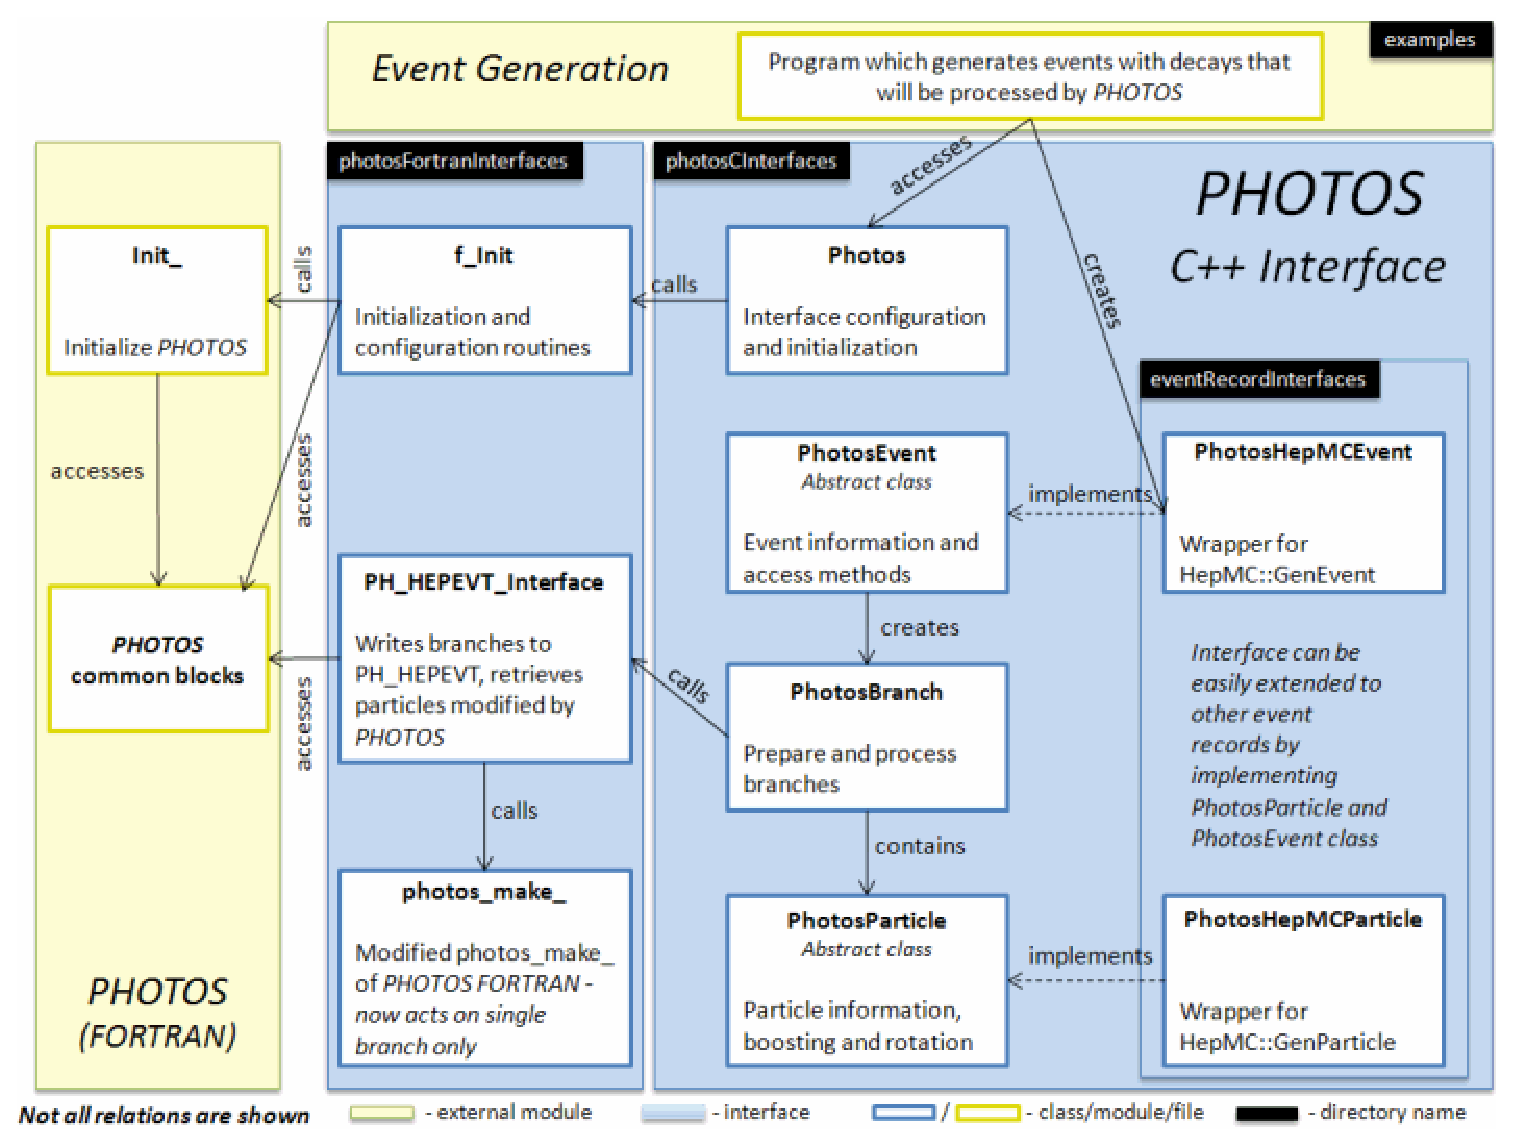
\includegraphics[scale=0.6]{interface_design.eps}
\label{fig:design}
\caption{{\tt PHOTOS} C++ interface class relation diagram}
\end{figure}

\begin{itemize}
  \item {\bf {\tt PHOTOS FORTRAN} Interface}\\
       This part of the code provides an interface 
       to the {\tt FORTRAN} library of {\tt PHOTOS}. In particular,
	   a wrapper for the routine which invokes the processing
	   of a single branch. Parts of the interface code are still left in {\tt FORTRAN}, but
	   can be rather easily rewritten to C++. 
       The most important part of this module, the {\tt PH\_HEPEVT\_Interface\_} class,
       is already implemented  in C++. This class is responsible for writing
	   the decay branch to be processed into the internal event record {\tt PH\_HEPEVT}.
       For further details regarding the interface to {\tt FORTRAN}
	   common blocks and routines see Appendix \ref{Interface to PHOTOS}.
  \item {\bf {\tt PHOTOS} C++ Interface} \\
       This is an abstract interface to the event record.
       The class {\tt PhotosEvent} contains information regarding the whole event
       structure, while {\tt PhotosParticle} stores all information regarding a single particle.
       All particles used by the interface are located in the event in the form of
       a list of {\tt PhotosParticle} objects.
       The last class located here, {\tt PhotosBranch}, contains information regarding
	 elementary branching to be processed by {\tt PHOTOS}.
  \item {\bf Event Record Interface} \\
       This contains the event record implementation classes. All classes stored here represent
       the implementation of specific event record interfaces and are responsible for reading,
       traversing and writing to the event record structure.
       Only the {\tt PhotosEvent} and {\tt PhotosParticle} classes must be implemented.
       The {\tt HepMC} event record interface is implemented
       through {\tt PhotosHepMCEvent} and {\tt PhotosHepMCParticle}. These classes are similar to the
       analogous {\tt TAUOLA} \cite{Davidson:2010rw} event record classes.
       An example of a minimalistic interface to an event record has been provided
       through the classes {\tt PhotosHEPEVTEvent} and {\tt PhotosHEPEVTParticle}\footnote{This interface is the only way of implementing NLO corrections in programs based on {\tt HEPEVT} event record}.
       %TP: we have to write something regarding the limitations of the HEPEVT interface
       They can be used as a template for a new interface to any other event record%
       \footnote{Thanks to the polymorphism, abstract part of the algorithm
       is well separated from the specific event record implementations.
       It even allows simultaneous use of several distinct event record implementations.}.
\end{itemize}

\subsection{Directory Structure}

\begin{itemize}
\item {\bf src/eventRecordInterfaces/ } - source code for classes which interface with event records.
      Currently only the {\tt HepMC} interface is located here.\\
  Classes:
  \begin{itemize}
  \item { \bf PhotosHepMCEvent} - interface to HepMC::GenEvent objects. 
  \item { \bf PhotosHepMCParticle} - interface to HepMC::GenParticle objects. 
  \item { \bf PhotosHEPEVTEvent} - interface to the event structure of the {\tt HEPEVT} format. 
  \item { \bf PhotosHEPEVTParticle} - interface to a single particle from the {\tt HEPEVT} event record.
  \end{itemize}   

\item {\bf src/photosCInterfaces/ } - source code for the general {\tt PHOTOS} interface.  \\
  Classes:
  \begin{itemize}
  \item { \bf Photos } - controls the configuration and initialization of {\tt PHOTOS}.
  \item { \bf PhotosEvent } - abstract base class for event information.
  \item { \bf PhotosParticle } - abstract base class for particles in the event.
  \item { \bf PhotosBranch } - contains one {\tt PhotosParticle}, and  pointers to its mothers and daughters.
  The filtering of branchings to be tried by {\tt PHOTOS} for photons emission is done here.
  \end{itemize}

\item {\bf src/photosFortranInterfaces/ } -  interface to {\tt PHOTOS FORTRAN} routines and common blocks. \\
  Files:
    \begin{itemize}
    \item { \bf f\_Init } - contains a wrapper for the {\tt PHOTOS FORTRAN} routines for initialization.
    \item { \bf PH\_HEPEVT\_interface } - contains a wrapper for accessing the
      {\tt  PH\_HEPEVT} common block.
    \item { \bf photos\_make.f } - contains  {\tt FORTRAN} routines to be  migrated to C++ rather soon.
    \item { \bf forW-ME.f } - c  {\tt FORTRAN} routines to calculate matrix element in W decay, own programming style.
    \item { \bf forZ-ME.f } - {\tt FORTRAN} routines  to calculate matrix element in Z decay, own programming style.
    \end{itemize}

\item {\bf src/utilities/ } - source code for utilities.\\
  Classes:
  \begin{itemize}
  \item { \bf Log} - general purpose logging class that allows filtering out output messages 
      of {\tt PHOTOS C++ Interface} and tracks statistics for each run.
  \item { \bf PhotosRandom} - random number generator taken from {\tt PHOTOS FORTRAN} and rewritten to C++.
  \end{itemize}   
\item {\bf src/photos-fortran/ } - {\tt PHOTOS FORTRAN} core rewritten to C++. Since version 3.54 {\tt PHOTOS} has been
      fully rewritten to C++ and located in its own namespace {\tt Photospp}\footnote{This means that no part of
      the code is shared with old {\tt PHOTOS FORTRAN} and both versions can be loaded simultanously without the
      risk of one version overwriting the options of the other.}. From the algorithmic point of view
full compatibility\footnote{The resulting modules are however not interchangeable and the program
 will not function if the {\tt PHOTOS FORTRAN} library is loaded instead of code encapsulated 
in {\bf src/photos-fortran/ } directory.
}
 with the {\tt FORTRAN } version is kept. The appropriate descriptions remain vaild;
in publications as well as in the code, now in C++.
  \item {\bf examples/ } - examples of different {\tt PHOTOS} C++ Interface uses.
    \begin{itemize}
        \item {\bf photos\_hepevt\_example} - stand alone example with a simple 
        $e^+e^- \rightarrow \tau^+\tau^-$ event written in {\tt HEPEVT} format
         and then processed by {\tt PHOTOS}.
	\item {\bf photos\_standalone\_example} - the most basic example which loads pre-generated 
	      events stored in a file in {\tt HepMC} format which are then processed by {\tt PHOTOS}.
	\item {\bf single\_photos\_gun\_example} - an example of using the {\tt processOne} method
	      to process only selected particles within the event record.
    \item {\bf photos\_pythia\_example} - an example of $e^+e^- \rightarrow Z \rightarrow \mu^+\mu^-$ events
	generated by {\tt PYTHIA 8.1} and processed by {\tt PHOTOS}. The analysis is done using {\tt MC-TESTER}.
    \item {\bf tauola\_photos\_pythia\_example } - an example of  {\tt TAUOLA} linked with {\tt PYTHIA 8.1}.
	The decay chain is processed by {\tt PHOTOS} and then analyzed with {\tt MC-TESTER}.
    \end{itemize}   
  \item {\bf include/} - directory for the header files.
  \item {\bf lib/ } - directory for the compiled  libraries. 
  \item {\bf documentation/ } - contains doxygen documentation and this latex file.
\end{itemize}

\subsection{Algorithm Outline}
\label{sect:Outline}

An overview of the algorithm for  the {\tt PHOTOS C++ Interface} is
given below. For clarity, the example assumes that the processed event
is stored in the {\tt HepMC} event record structure.

The first step is creation of a {\tt PhotosHepMCEvent} object from
a {\tt HepMC::GenEvent} event record. After that, the {\tt process()} method should
be executed by the user's code\footnote{Instead of creating a {\tt PhotosHepMCEvent} and processing the whole event,
a user may want to execute {\tt Photos::processParticle(...)} or {\tt Photos::processBranch(...)}
for branching or branch, where {\tt PHOTOS} is expected to perform its tasks.
For details see Appendix~\ref{PHOTOSgun}.
}, invoking the following process:

\begin{enumerate}
\item The {\tt HepMC} event record is traversed and a list of all decaying
      particles is created.
\item Each particle is checked and if the resulting branching is a self-decay\footnote{A history entry in the event record, like
      $Z\to Z$ or $\tau \to \tau$.} it is skipped.
\item For each remaining particle a branching  including the particle's mothers and daughters
      is created. Special cases consisting of mothers and daughters but without  intermediate particle 
to be decayed are also added to the 
	  list of branchings.
\item Branchings are filtered out again, this time with  the user's choice of processes
      to be skipped by the photon adding algorithm.
\item Each branching  is processed by {\tt PHOTOS} separately:

	\begin{enumerate}
  
	\item The branching is written to {\tt PH\_HEPEVT}
	\item The {\tt PHOTOS} photon adding algorithm is invoked 
 	\item The resulting branching is taken back from {\tt PH\_HEPEVT} and any changes made by {\tt PHOTOS}
	      to the already existing particles and their whole decay trees are integrated into the event record.
	\item Finally, the created photons are added to the event record.
	\end{enumerate}

\end{enumerate}

The underlying HepMC::GenEvent is hence modified with the  insertion of photons.

\section{Extensibility}
\label{sec:extensibility}
 The purpose of the present version of the C++ interface to {\tt PHOTOS} is to enable 
all the functionality of its {\tt FORTRAN} predecessor to be available for the HepMC data
structure. Some methods for improved initialization are already introduced in this version. The new program 
functionality has been prepared to enable further extensions in the future. 
Let us briefly discuss some of these points.

\subsection{{\tt PHOTOS} Extensions}
In this paper we have presented an algorithm as it is today. 
That is, a version which is compatible with the one implemented in {\tt FORTRAN}.

\begin{itemize}


\item
As can be seen from the text presented, we have prepared the structure 
for the implementation of channel dependent matrix elements. This work, requiring
special modifications to the {\tt FORTRAN} code and  applicable one at a time only can  
be simply integrated all together into the C++ version. This is not urgent.
 We are  not convinced if such complication is worth 
the inconvenience for the user as it requests more strict control of the event 
record content. The gain of precision is 
not that important because the precision is already quite good. 
This is why we have not incorporated  these auxiliary upgrades to C++ already now.
Instead, as an intermediate step, we developed validation techniques
for the program. These are required prior to a re-write of the
numerically sensitive part of the program (which is algorithm-wise
rather simple) anyway.

\item
Methods devised to check the content of HepMC as used by {\tt PHOTOS} are
described in Appendix \ref{App:Logging}. 
They need to be used whenever {\tt PHOTOS} 
processes events from a new generator e.g. upgraded versions of  {\tt PYTHIA},
which may fill the event record in an unexpected way.
Experience gained from many years of developing and maintaining the algorithm
have shown, that this is the most demanding task; the necessity to
adapt to varying physics and technical input of the event record pose
a multitude of problems. The nature of these difficulties cannot be
predicted in advance. 

\item
For the sake of debugging we have introduced new control methods 
and ones which activate
internal printouts of the {\tt FORTRAN} part of the code.
The routine {\tt PHLUPA} \cite{Barberio:1993qi} can be activated  to verify 
how an event is constructed/modified, and to investigate energy 
momentum (non-) conservation or other inconsistencies.
This is quite convenient, for example, for tracing problems in the
information passed to {\tt PHOTOS}.


\item
Numerical stability is another consideration; it cannot be separated from
physics constraints. The condition  $E^2-p^2=m^2$ may be broken  because of 
rounding errors.  However, due to intermediate particles with
  substantial widths, the on mass shell condition may not be applicable.
{\tt PHOTOS} may be adapted to such varying conditions, but it requires
good interaction with users. The protection which removes 
inconsistencies in the event record may be a source of unexpected difficulties
in the other cases. 
At present, such methods are left in the {\tt FORTRAN} part of the algorithm, 
which
will be gradually reviewed and  migrated to C++.
\end{itemize}

 
\subsection{Event Record Interface}
In the times of {\tt FORTRAN}, the {\tt PHOTOS} interface used an internal event structure which was
based on {\tt HEPEVT},
adding to it (understood as a data type) an extra variable defining 
the status of particles with respect to QED Bremsstrahlung. In some cases, like
$\tau \to l \nu_l \nu_\tau$, bremsstrahlung was already generated earlier
by other generator, and {\tt PHOTOS} should not be activated on such decays.
At present, instead, a set of initialization methods is 
prepared as described in Appendix \ref{section:suppress}. 

There is definite room for 
improvement. For example if the vertex $q \bar q \to l^\pm l^\mp g$ is encountered
(note the presence of $g$ in the final state),
the interface could `on the fly' add an intermediate $Z$ into the record and enable {\tt PHOTOS}
on the temporarily constructed decay branching, $Z \to l^\pm l^\mp $. 

Internally, in the {\tt FORTRAN} part of {\tt PHOTOS}, the data
structures based on {\tt HEPEVT}: {\tt PH\_HEPEVT} and {\tt PHOEVT}, 
are used, but they store only a single elementary decay. 
At this step in the program
evolution it might not be the most elegant solution, but it prevents
the need to redo many of the {\tt FORTRAN} era benchmarks.






\section{Testing}
\label{sec:tests} 
One of the most important parts of the {\tt PHOTOS} project are its physics oriented tests.
Several domains
of physics tests should be mentioned. Users interested in precision 
simulations of Z or W decay  will 
find  the papers \cite{Nanava:2009vg,Golonka:2006tw,Golonka:2005pn}
most interesting. There, careful comparison with the first order matrix element 
and confirmation of the agreement is concluded first.
For $Z$ decays, comparisons  with Monte Carlo program based on exclusive 
exponentiation with up to second order matrix element
is possible and was performed on some benchmark distributions.
Inclusion of a correcting weight was found to be numerically less important
than absence of the second order matrix element in the YFS exponentiation scheme. 
In these comparisons the Monte Carlo programs from LEP times 
\cite{koralz4:1994,kkcpc:1999} were used. In numerical tests {\tt MC-TESTER} \cite{Davidson:2008ma}
was used. The advantage of the method is that C++ and {\tt FORTRAN} program
results can be easily compared\footnote{We thank Andy Buckley for checking numerically
 that our conclusions on the first order exact YFS exponentiation results extend
to the programs presently used at the LHC such as  
SHERPA and HERWIG++.  }.
 
For inclusive calculations, FSR radiative corrections are at the one permille level.
For semi-inclusive cross sections, such as the total rates of Z decay for events
where the hardest photon energy (or two hardest photon energies)   exceed 1 GeV in the Z rest frame, differences
between results from {\tt PHOTOS} ({\tt PHOTOS}  without the matrix element correcting weight)
and YFS based generators of the first or second order were also 
at the 0.2 \% level. 
On the other hand, if two  hard photons were requested and invariant masses constructed from leptons
and hard photons were monitored,
 the level of differences exceeded 
 30 \%. However, even in this region of phase space {\tt PHOTOS},  without the correcting
weight, performs better\footnote{In 
  the phase space region were only one hard photon is tagged this conclusion seems to depend
  on the variant of exponentiation in use, \cite{koralz4:1994} or \cite{kkcpc:1999}.
                                }
than programs based on exponentiation and the first order matrix element only. 

This conclusion needs to be investigated if   
realistic experimental 
cuts are applied. Fortunately the necessary programs are available for Z decay.
In the case of $W$ decay, second order Monte Carlo generators supplemented with 
exponentiation are not available at this moment.
 
For users interested in the simulation of
background for Higgs searches at the LHC and for any other applications where 
two hard photon configurations are important, studies based on the comparison with 
a double photon matrix element are of 
interest. For {\tt PHOTOS} Monte Carlo such tests were initiated 
in refs.~\cite{Barberio:1993qi,RichterWas:1994ep,RichterWas:1993ta}.
Finally, users interested in low energy processes where the underlying physics model 
for photon emission cannot be controlled by theory sufficiently well
(scalar QED may 
be considered only as the starting point), will profit 
from \cite{Nanava:2006vv,Nanava:2009vg}. In all cases it is important that
the  program generation cover the full phase-space and that there are no 
approximations in phase-space. As in the {\tt FORTRAN} version, the code 
features approximation in the kernel. In some cases the process dependent 
complete first order 
kernel is available but it is not always installed in the public version,  
because the resulting approximation is 
numerically unimportant and requires control of the spin state for the decaying 
particle. This requires better control of the event record than what was available 
in {\tt FORTRAN}. At present such an option is prepared (see Section \ref{sect:F77fill}) for $W$ and $Z$ decays. It is also available for the two body decays of scalar into scalars. Then, exact mean exact with respect to scalar QED only. 

The main purpose of the present paper is program documentation. That is why
we also need to cover the program tests required to guarantee its proper installation.
The physics tests discussed above 
do not guarantee that the program will perform well on a particular platform and installation. Tests and debugging of the installation
are necessary too.  If the content of the event record is non-standard or rounding errors are large, the performance of {\tt PHOTOS} will deteriorate.


The first check after installation of {\tt PHOTOS} is whether some energy momentum non 
conservation appears. Such offending events should be studied
before {\tt PHOTOS}  and after {\tt PHOTOS} is run to modify them.
If it is impossible to understand why inconsistencies for energy momentum non 
conservation were created by {\tt PHOTOS}, the authors should be contacted. Sometimes
monitoring how an event is constructed inside the {\tt FORTRAN} part of the code
may be useful. For that purpose the steering of monitoring\footnote{See Appendix \ref{App:Logging}
for the command {\tt Log::LogPhlupa(int from, int to)}}
 is
available from the C++ part of the code. In practice only rather
 advanced users will profit from the printouts. However, it may be sent to
the authors and help to quickly identify the cause of the problems.


The next step in benchmarking relies on comparisons with benchmark distributions. 
At present, we store these tests with the help of {\tt ROOT} \cite{Antcheva:2009zz} and our {\tt MC-TESTER} program \cite{Davidson:2008ma}.



\subsection{{\tt MC-TESTER} Benchmark Files}



Over years of development of the {\tt TAUOLA} and {\tt PHOTOS} programs a certain level 
of the automation of tests was achieved. It was found that monitoring all the invariant mass distributions which can be constructed out of a given decay represent 
a quite restrictive but easy to implement test.
Finding the relative fraction of events for each distinct final state 
 complemented that test and is implemented now in the public version of {\tt MC-TESTER}. 
We have applied this method 
for {\tt PHOTOS} too. In this case, some soft final state particles have to be ignored because we are bound to  work with  samples which otherwise would
exhibit properties of unphysical infrared regulators (see Section 6.1 of 
ref \cite{Davidson:2008ma} for more details). For the most popular 
decays the benchmarks are collected on our project web page \cite{Photos_tests}.
In our distribution, we have collected numerical results in the directory
{\tt examples/testing} and its subdirectories:  
{\tt Htautau, ttbar, Wenu, Wmunu, Zee and Zmumu}. Each of them includes
an appropriate initialization files for the particular run of {\tt PYTHIA}. Numerical results from long runs of {\tt MC-TESTER} based tests
are stored for reference\footnote{Details on the initialization for the 
runs are given in 
{\tt README-benchfiles}.}. At present, our choice of tests is oriented toward 
the LHC user and radiative corrections in decay of W's, Z's and Higgs particles.
Most of the users of low energy experiments use the {\tt FORTRAN} version 
of the code, which is why our tests and examples for the C++ version are not geared toward 
low energy applications.


\subsection{Results}
\label{sec:results}
In principle, for the algorithm of  photon(s) construction, the C++ interface of
{\tt PHOTOS} introduces nothing new with respect to the 
version of {\tt PHOTOS} as available in {\tt FORTRAN}.
That is why the  tests which are collected in \cite{Photos_tests} are not
recalled here, they were only reproduced and found to be consistent with the ones for
old {\tt PHOTOS FORTRAN}.
However the algorithm for combining a modified branching, including the added 
photon(s), to the rest of the event tree was rewritten.
Examples of spin dependent observables are of more interest because they test this new part of the code.
The $\pi$ energy spectrum in the decaying
Z boson rest-frame is the first example. 
The $\pi^\pm$ originates from $\tau^\pm \to \pi^\pm \nu $ decay and, 
as was already shown a long time ago \cite{Boillot:1988re}, its energy spectrum is modified by bremsstrahlung both in $\tau$ and $Z$ decays. The net
bremsstrahlung  effect is similar to the one of e.g. Z polarization. In Fig.~\ref{fig:KKMC} this result is reproduced.

Let us now turn to tests using observables which are sensitive to
transverse spin effects.  For that purpose we study the decay chain:
$H\to \tau^+\tau^-$, $\tau^\pm \to \rho^\pm \nu_\tau$, $\rho^\pm \to
\pi^\pm \pi^0$, where {\tt PHOTOS} may act on any of the branchings
listed above. An inappropriate action of the C++ part of {\tt PHOTOS}
could result in faulty kinematics, manifesting itself in a failure of
energy-momentum conservation checks of the event record or faulty spin
correlation sensitive distributions. However, as we can see from Fig.~\ref{fig:acoplanarity},
 the distributions (as they should be) remain nearly identical to the ones given in
\cite{tauolaC++,Davidson:2010rw}. The emission of soft and/or
collinear photons to the $\tau^+$ or $\tau^-$ does not change the
effects of spin correlations. The kinematical effects of hard,
non collinear  photons are responsible for dips in 
the acoplanarity distributions at $0$, $\pi$ and $2\pi$.

\begin{figure}[h!]
\centering
\subfigure[bremsstrahlung from  $\tau^+ $ decay only]{
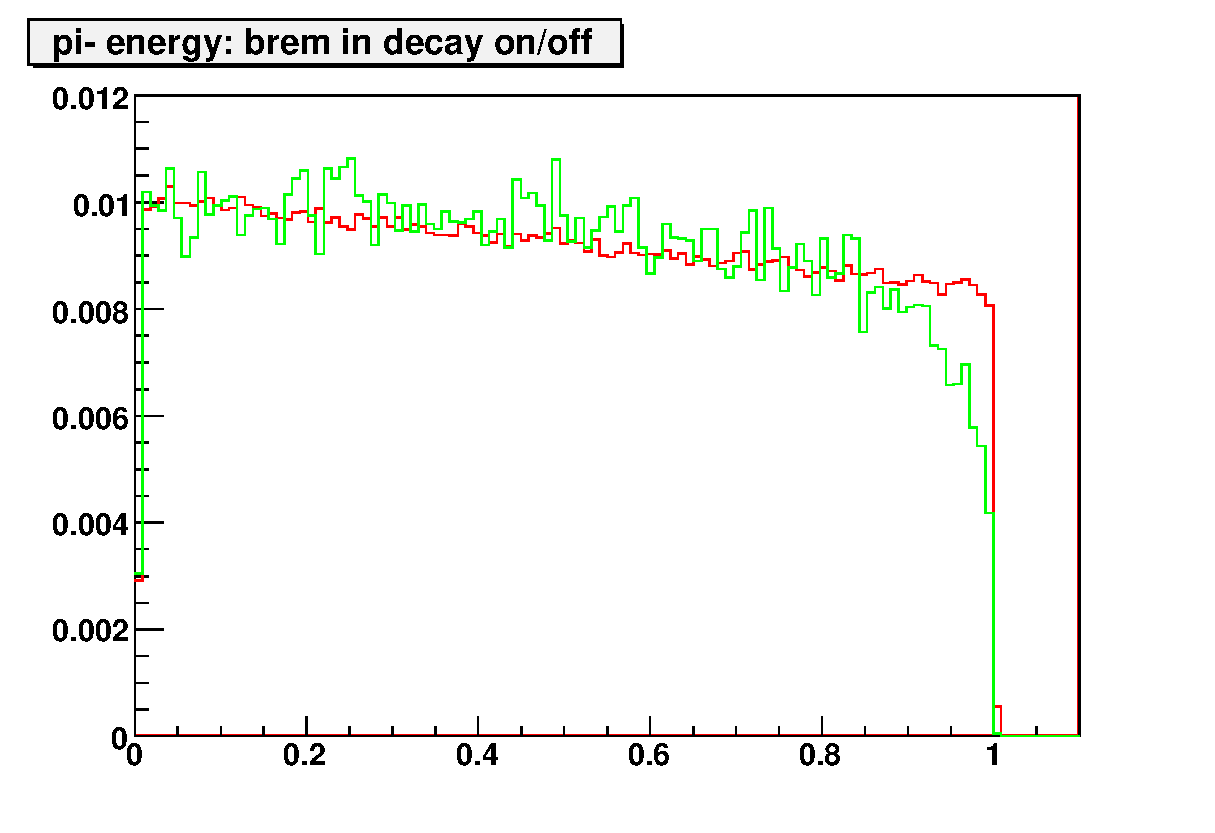
\includegraphics[scale=0.35]{bremdec.eps}
}
\subfigure[bremsstrahlung from $Z$, $\tau^+ $ and $\tau^- $ decays]{
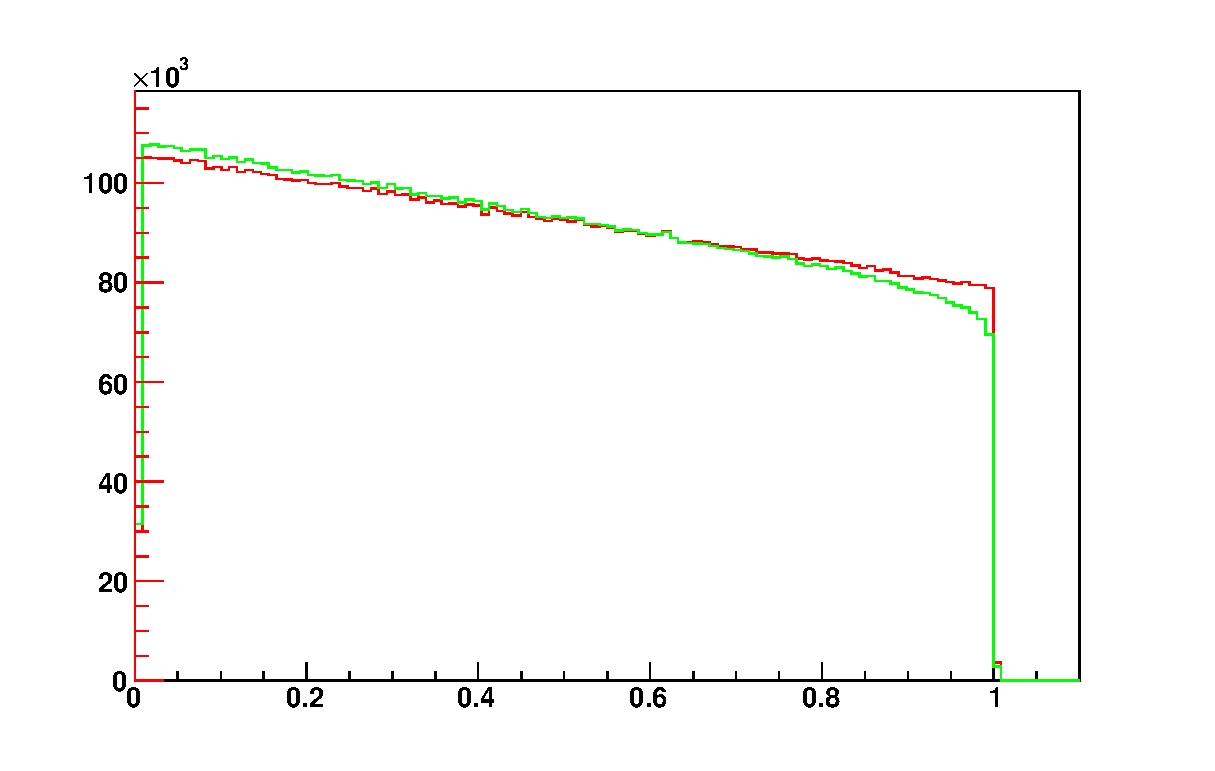
\includegraphics[scale=0.35]{bremall.eps}
}
\caption{ Bremsstrahlung effects for longitudinal spin observables
for the cascade decay: $Z \to \tau^+ \tau^-$, $\tau^\pm \to \pi^\pm\nu$.
$\pi^+$ energy spectrum in the Z rest-frame  is shown. The red line is for 
bremsstrahlung switched off
and green (light grey) when its effect is included. 
In the left plot, bremsstrahlung is in $\tau^+ $ decay only.
In the right plot, bremsstrahlung from $Z$ and  $\tau^\pm$ decays is
taken into account.
These plots have been prepared using a custom {\tt UserTreeAnalysis} of {\tt MC-TESTER}.
They  can be recreated with the test located in the {\tt examples/testing/Ztautau} directory, see  {\tt examples/testing/README-plots} for technical details. Results are 
consistent with Fig.~5 of Ref.~\cite{Eberhard:1989ve}.
\label{fig:KKMC}
}
\end{figure}
\begin{figure}[h!]
\centering
\subfigure[selection C]{
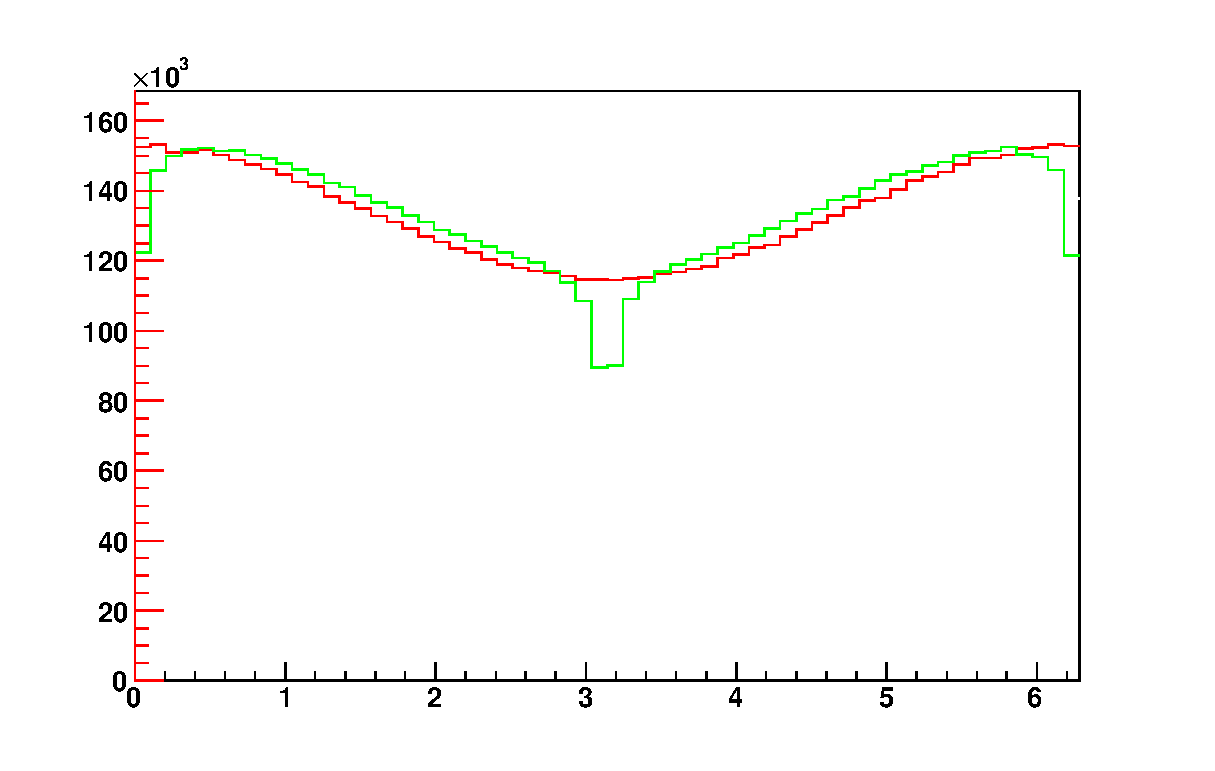
\includegraphics[scale=0.35]{coplanarity-angle-C-photon-over-1-GeV.eps}
}
\subfigure[selection D]{
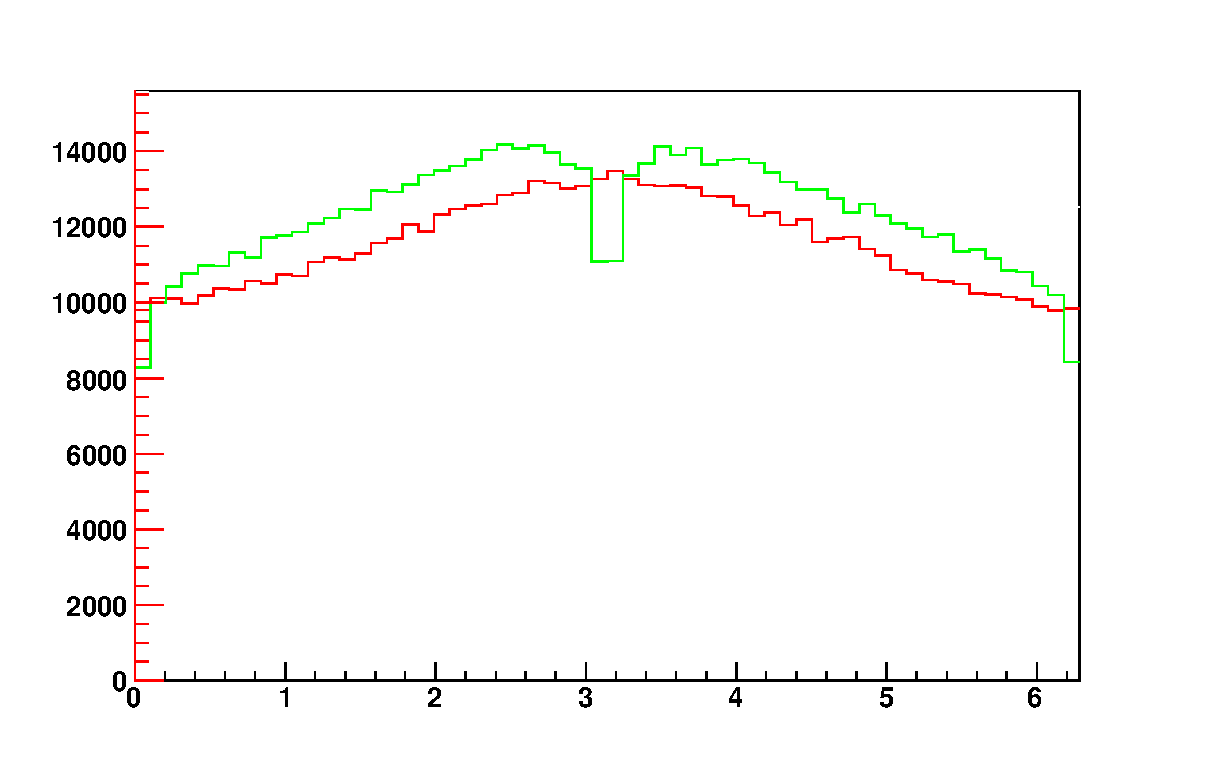
\includegraphics[scale=0.35]{coplanarity-angle-D-photon-over-1-GeV.eps}
}
\caption{Bremsstrahlung effects for transverse spin observable: 
  The distribution of the acoplanarity angle of oriented planes spanned respectively on 
  the $\pi^+\rho^+$ and $\pi^-\rho^-$ momenta is shown.  
The distribution is defined in the rest frame of the
  $\rho^+ \rho^-$ pair for the scalar Higgs decay chain $H\to
  \tau^+\tau^-$, $\tau^\pm \to \rho^\pm \nu_\tau$, $\rho^\pm \to
  \pi^\pm \pi^0$. {\tt PHOTOS} is used to generate
  bremsstrahlung.  The red curve indicates the distribution when
  bremsstrahlung effects are ignored and for the green curve (light grey) 
only events
  with bremsstrahlung  photons of energy larger than 1 GeV
  in the $H$ rest frame are taken. For the definition of selections C
  and D see.~\cite{Bower:2002zx,Desch:2003rw}.  These plots have been created using
  a custom {\tt UserTreeAnalysis} of {\tt MC-TESTER}.  They can be
  recreated by  the test located in the {\tt
    examples/testing/Htautau} directory, see {\tt
    examples/testing/README-plots} for technical details.
\label{fig:acoplanarity}
}
\end{figure}


In Ref.~\cite{Adam:2008ge} a discussion of the systematic errors for the measurement of the Z cross 
section at the LHC is presented. One of the technical tests of our software is to obtain
Fig. 1b of that paper. In our Fig.~\ref{fig:lineshape} we have 
reproduced that plot using {\tt PYTHIA 8.1} and {\tt PHOTOS}. Qualitatively, the effect
of FSR QED bremsstrahlung is in the two cases quite similar. 


In  Fig.~\ref{fig:lineshape} we present a plot of the bare electron pair 
(which means electrons are not combined with the collinear photons that accompany them) from $Z$
 decay with and without {\tt PHOTOS}. It is similar to
the plots shown for {\tt Horace} or {\tt Winhac}; see Refs.~\cite{CarloniCalame:2003ux,Winhac} and related
studies.
One should bear in mind that this is again a technical test with little 
direct application to physics. As explained in the figure caption, the LHC production process was used.
\begin{figure}[h!]
\centering
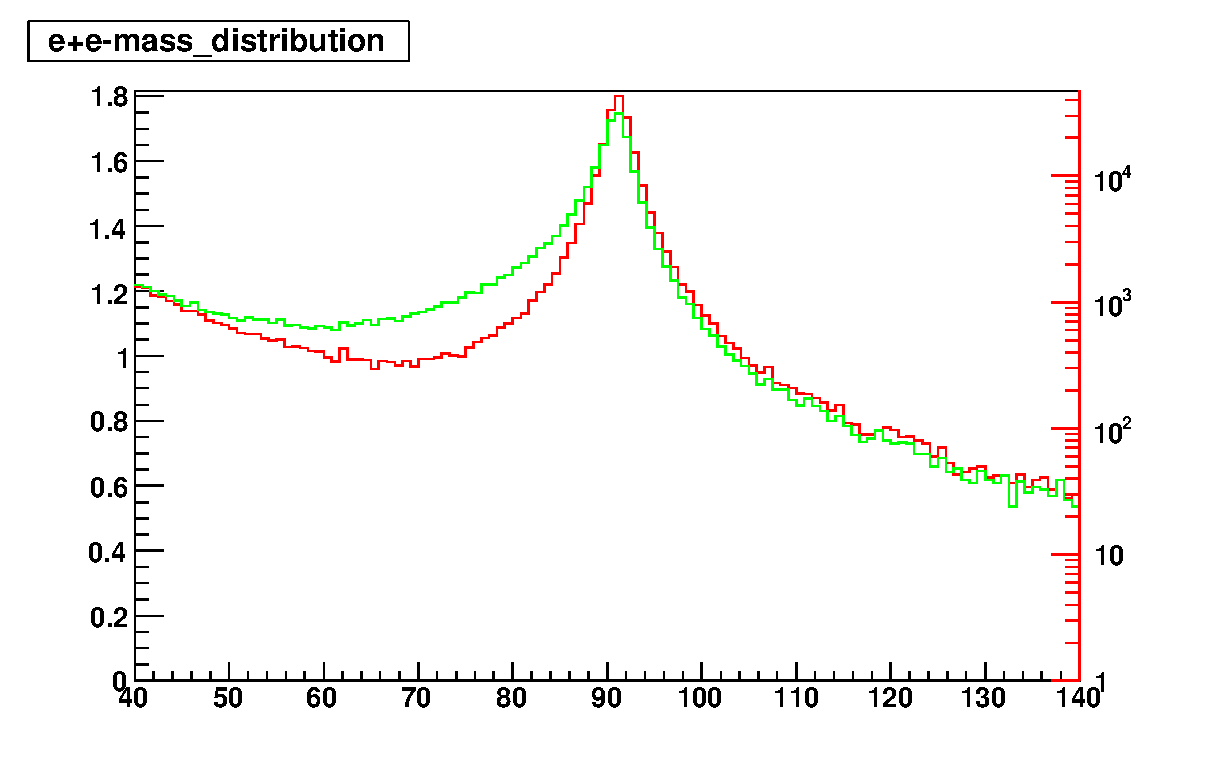
\includegraphics[scale=0.85]{lineshape.eps}
\caption{Distribution of the bare $e^+e^-$ invariant mass. The green curve 
(light grey) represents results when final state 
bremsstrahlung is generated (with the help of {\tt PHOTOS} Monte Carlo). For the red curve FSR 
bremsstrahlung is absent. The event sample is generated with the help of {\tt PYTHIA 8.1}.
The simulation of pp collisions at 14 TeV center-of-mass energy is performed.
The $Z/\gamma$ mediated hard process is used.
This plot has been created using a custom {\tt UserTreeAnalysis} of {\tt MC-TESTER}.
It can be recreated with the test located in the {\tt examples/testing/Zee} directory, see  {\tt examples/testing/README-plots} for technical details.
\label{fig:lineshape}
}
\end{figure}



We have also checked that {\tt PHOTOS} works for $t \bar t$ events and the simulations explained in \cite{RichterWas:1993ta} can be repeated.
For this purpose we have produced $t \bar t$ pairs in $pp$ collisions at 
14 TeV center-of-mass energy. We have produced rates for events with zero, one or
at least two photons of energy above 0.001 of the $t \bar t$ pair mass
(energies are calculated in  the hard scattering frame).
Results are given in the following table which is constructed from  
$gg \to t \bar t$ events only:


\vspace{0.3cm} 
\begin{center}
{ \begin{tabular}{c c} 
\toprule 
Final state &  Branching Ratio (\%) $\pm$ Statistical Errors (\%) \\  
\midrule
{$ \widetilde{t} t \; \;\; \;$}  &  {99.0601 $\pm$ 0.0315}  \\ 
%\hline 
 {$  \widetilde{t} t \gamma \;\;$} &   { 0.9340 $\pm$  0.0031}   \\ 
%\hline 
{$  \widetilde{t} t \gamma \gamma$}  &  { 0.0060 $\pm$  0.0002}  \\ 
\bottomrule
\end{tabular} 
}  
\end{center} 

10 million events were generated and a slightly modified 
version of {\tt MC-TESTER}'s {\tt LC-analysis} from Ref.~\cite{Golonka:2002rz}
was used for calculation of the event rates\footnote{  We do not supplement the list of 
final state particles with the second mother, in contrast to the choice used in {\tt LC-analysis} from  Ref.~\cite{Golonka:2002rz}. }.
{\tt ROOT} files for differential distributions are 
collected in the directory {\tt examples/testing/ttbar}. 

\subsection{Tests Relevant for Physics Precision}


Let us now turn to an example of the test for the two photon final state configuration.
We compare (i) KKMC \cite{kkcpc:1999} with exponentiation and second order matrix element (CEEX2), (ii) KKMC with exponentiation and first order matrix element (CEEX1)
and finally (iii) the results of {\tt PHOTOS} with exponentiation activated. As one can see from the table below, the rates 
coincide for the three cases up to two permille for the event configurations 
where zero, one or at least two photons of energy above 1 GeV are accompanying the $\mu^+\mu^-$ pair.

\begin{table}
\centering 
\begin{tabular}{lrrr} 
\toprule 
Decay channel &\multicolumn{3}{c}{ Branching Ratio $\pm$ Rough Errors   (100M event samples)} \\ 
      & {KKMC CEEX2} (\%) & {KKMC CEEX1} (\%)& {\tt PHOTOS} exp. (\%)\\ 
\midrule
 {$Z^{0} \rightarrow \mu^{+} \mu^{-} $} & {83.9190 $\pm$  0.0092} &{  83.7841 $\pm$  0.0092} & 83.8470 $\pm$ 0.0092\\ 
%\midrule
 {$Z^{0} \rightarrow \gamma \mu^{+} \mu^{-} $} & {14.8152 $\pm$  0.0038} &{  14.8792 $\pm$  0.0039} & 14.8589 $\pm$ 0.0039 \\ 
%\midrule
{$Z^{0} \rightarrow \gamma \gamma \mu^{+} \mu^{-} $} & { 1.2658 $\pm$  0.0011} &{   1.3367 $\pm$  0.0012} & 1.2940 $\pm$ 0.0011\\ 
\bottomrule
\end{tabular}
\end{table}

Agreement at this level is not seen in the differential distributions, see Fig.~\ref{fig:gamgam}. For example the spectrum of 
the two photon mass is quite different between the first and second order 
exponentiation result. This is of potential interest for background simulations 
for $H \to \gamma \gamma$. In contrast, the difference between the results from {\tt PHOTOS} and CEEX2 are much smaller. {\tt PHOTOS} exploits the first order matrix element 
in a better way than exponentiation. As a consequence it reproduces terms resulting in second order leading logarithms. This observation is important not only for 
the particular case of $Z$ decay but for the general case of double bremsstrahlung in any decay as well.

\begin{figure}[h!]
\centering
\subfigure[CEEX2: red; CEEX1: green]{
\includegraphics[scale=0.35]{{M1@0001.eps}}
}
\subfigure[ CEEX2: red; PHOTOS: green]{\label{plot:b}
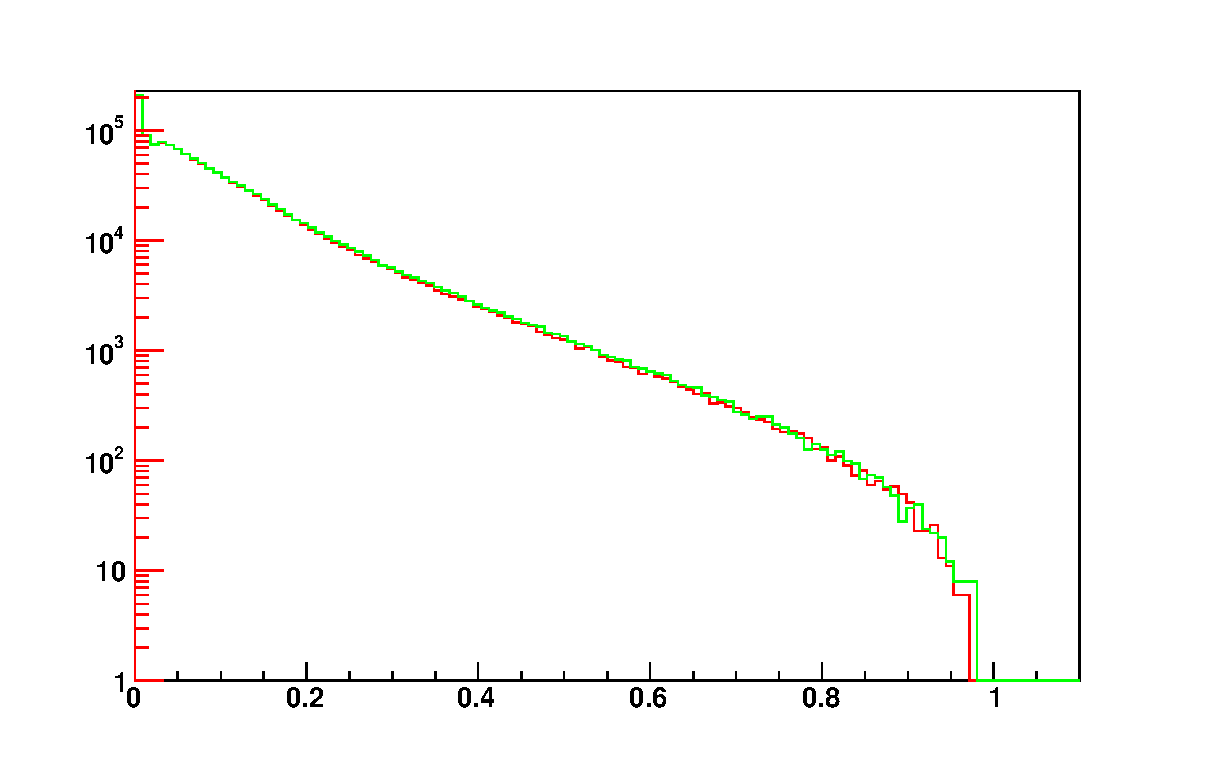
\includegraphics[scale=0.35]{b-M1@0001.eps}
}
\caption{ The spectrum of the $\gamma \gamma$ invariant mass in $Z \to \mu^+\mu^-$
decay. Events with two hard photons, both of energy above 1 GeV in the $Z$ rest 
frame are taken. Comparisons are shown for CEEX2 and CEEX1 (left plot), and CEEX2 and {\tt PHOTOS}
(right plot). The prediction from {\tt PHOTOS} is clearly superior for applications aimed at
the simulation of Higgs boson backgrounds. In the case of solutions based on YFS 
exponentiation, the second order matrix element must be taken into account. Fig.~\ref{plot:b} was obtained
from our example, {\tt examples/testing/Zmumu}, after adaptation of the center-of-mass energy 
(91.17 GeV) and test
energy threshold (1 GeV). Samples of 100 million events were used. 
See  {\tt examples/testing/README-plots} for technical details. Reference 
{\tt ROOT} files for KKMC CEEX samples are, however, created outside of the distribution.
  \label{fig:gamgam}
}
\end{figure}


The numerical results collected here provide part of the program benchmarks. 
They are of limited but nonetheless  of  some physics interest as well.
 {\tt PHOTOS} provides only one step in the simulation chain: 
bremsstrahlung in decays or final state bremsstrahlung. One can ask 
the question of whether such a specialized unit is of interest and whether it is not better 
to provide the complete chain for ``truth physics simulation'' as a single simulation package. Obviously, this will
depend on particular needs. Final state QED corrections can be 
 separated from the remaining genuine electroweak corrections and 
in particular the initial state QED bremsstrahlung from quarks. 
One should bear in mind, that final state bremsstrahlung 
needs to be disentangled from detector acceptance dependencies and is not of 
interest in itself. This must be done e.g. to measure the properties of weak bosons.

One should bear in mind that even for QED FSR alone, the discussion of the physics 
precision of the simulation result requires further checks. In the case of 
$Z$ decays, Refs.~\cite{Golonka:2005pn,Golonka:2006tw} may not be enough.
With increasing precision, the estimation of uncertainty becomes dependent on 
the particular choice of details for the experimental cuts. Comparisons of different
calculations become important too. A good example of such work in the conext of 
other measurements can be found in Refs.~\cite{Jadach:1995pd,Arbuzov:1996eq}; 
for the simulation of 
FSR QED corrections, the Monte Carlo programs collected for {\tt PHOTOS} generator 
tests are probably enough. 
A discussion of QED initial final state interference may follow the strategy presented
in \cite{Jadach:1999gz}. There, the question of experimental cuts must be included 
as well. Once these steps are completed, discussion 
of complete electroweak corrections in the context of realistic observables should 
be simplified.



Genuine weak corrections have to be taken into account separately.
Such solutions may be possible,  if together with the {\tt PHOTOS Interface},
 weak corrections are provided for example with the help of the {\tt TAUOLA Interface}.
A discussion
of the complete electroweak corrections, as shown in Fig. 1a of  \cite{Adam:2008ge},
is not the purpose of our document. Let us point out however that electroweak 
non-QED corrections can be in principle installed into the {\tt PYTHIA 8.1} + {\tt PHOTOS} simulation with 
the help of the e.g. {\tt TAUOLA} interface \cite{Davidson:2010rw}.
But for such a solution to be precise, further work is needed \cite{Bardin-private}.

Sizeable initial state QED corrections are usually embodied in  units 
simulating parton showers. This may need some experimental analysis as well. 
Recently experimental data from LEP1 times were revisited by the DELPHI collaboration \cite{Abdallah:2010tk}.
Tension between data and the theoretical description is 
mentioned. This may mean that the description of initial state QED bremsstrahlung 
at the LHC will need to be re-investigated with the help of LHC data as well.
That is also why it  might be useful to keep initial state QED, final state QED and their interference corrections in separate modules. 

We leave such estimations of the theoretical uncertainty for $Z$ and $W$ 
production at the LHC 
to the forthcoming research, where a realistic choice of experimental conditions and
observables 
will become an integrated part. \vskip -2 mm

\section{Summary and outlook}
\label{sec:summary}
We have presented a new version  of {\tt PHOTOS} Monte Carlo. The part of 
{\tt PHOTOS} which operates on 
event records is now rewritten into C++ and uses the HepMC event record 
format for input and output. The physics performance of the program is the
same as that of the {\tt FORTRAN/HEPEVT} version, but better steering options are introduced. 
Also, when an elementary decay is to be modified by {\tt PHOTOS}, 
it is first transformed to its rest frame. The $z$-axis is orientated along the decaying particle's mother's direction, as seen in this rest  frame. Such modification is 
necessary to calculate process dependent kernels
featuring the complete first order matrix element. If the interest will arise,
the appropriate kernels explained in
Refs.~\cite{Golonka:2006tw,Nanava:2006vv,Nanava:2009vg} can be installed
into the C++ version of {\tt PHOTOS}. The necessary information is extracted
from the event record and can be used.
At present some parts of the algorithm are left in {\tt FORTRAN}.
 This remaining {\tt FORTRAN} part of the code 
can be recoded to C++ rather easily, but the necessary numerical tests 
are time consuming. That is why we have left these changes for later 
releases. 

{Finally let us point to ref.~\cite{Arbuzov:2012dx}. Thanks to this work, for LHC applications in $Z$, $W$ decays,
{\tt PHOTOS} Monte Carlo systematic error was established at  0.3\%, even   0.2\% for the case of matrix element correction activated. The estimation is valid
for complete final state radiative corrections, not for photonic bremsstrahlung
alone.
}

\vskip 2 mm

\centerline{\large\bf Acknowledgements}


Useful discussions with P. Golonka during the early stage of project development and discussions 
with members of the ATLAS and CMS collaborations and the LCG/Genser team 
are acknowledged.
%We are especially indebted to the pilot users of the interface.
%, in particular to:
%nd-fix


Partial support by the Polish-French collaboration
no. 10-138 within IN2P3 through LAPP Annecy and 
during the final completion of this work is
also acknowledged.



\bibliography{Photos_interface_design}{}
% \bibliographystyle{plain}
\bibliographystyle{utphys_spires}





%------------------------------------------------------------------------------
\newpage
\appendix

\section{Appendix: Interface to {\tt PHOTOS FORTRAN}}
\label{Interface to PHOTOS}


This appendix is addressed to developers of the interface,
and special users interested in advanced options of {\tt PHOTOS}.
The discussed below {\tt COMMON} blocks of {\tt FORTRAN} were used in the
program up  to version 3.53 only.
Starting from version 3.54 some of these {\tt COMMON}  blocks were preserved,
as the struct objects of C. The following ones may be of some interest for the
user:
{\tt PHOCOP, PHOKEY, PHOSTA, PHLUPY}.

Names of variables and structs are not modified with respect to {\tt FORTRAN}, 
the  C++ definition style is adapted, small letters are used and underscore is added at the
end of structs names.
Common {\tt HEPEVT} is preserved for use of example and future applications,
 where the main program is in {\tt FORTRAN}.
The interface is available
through the classes {\tt PhotosHEPEVTEvent.h} and {\tt PhotosHEPEVTParticle.h}.
Internally in C++  {\tt Photos} code, the {\tt HEPEVT}-like  data type
is used.

\subsection{Common Blocks}

In the following let us list the common blocks of {\tt PHOTOS} which are accessed
from C++.

\begin{description}
\item[PHOCOP] coupling constant and related parameters.
    \begin{description}
	\item[ALPHA]  \textit{double} coupling constant $\alpha_{QED}$.
	\item[XPHCUT] \textit{double} minimal energy (in units of half of the decaying particle's mass) for photons to be explicitly generated.
    \end{description}
\end{description}

\begin{description}
\item[PHOKEY] keys and parameters controlling the algorithm options.
    \begin{description}
	\item[FSEC]   \textit{double} internal variable for algorithm options, the default is FSEC=1.0\; .
	\item[FINT]   \textit{double} maximum interference weight.
	\item[EXPEPS] \textit{double} technical parameter, blocks crude level high photon multiplicity from configurations less probable than EXPEPS, the default is $10^{-4}$.
	\item[INTERF] \textit{bool} key for interference, the matrix element weight.
	\item[ISEC]   \textit{bool} switch for double bremsstrahlung generation.
	\item[ITRE]   \textit{bool} switch for bremsstrahlung generation up to a multiplicity of 4.
	\item[IEXP]   \textit{bool} switch for exponentiation mode.
	\item[IFTOP]  \textit{bool} switch for photon emission in top pair production in quark (gluon) pair annihilation.
	\item[IFW]    \textit{bool} switch for leading effects of matrix element in leptonic W decays.
    \end{description}
\end{description}

\begin{description}
\item[PHLUPY] debug messages handling.
    \begin{description}
    \item[IPOIN]  \textit{int} messages above this value will not be displayed.
	\item[IPOINM] \textit{int} messages below this value will not be displayed.
    \end{description}
\end{description}

\begin{description}
\item[PH\_PHOQED] supplement for the PH\_HEPEVT event record to block emission 
from some particles.
    \begin{description}
    \item[QEDRAD[ 10000]]  \textit{bool} flag enabling a {\tt FORTRAN} users
    to block emission from particles stored in PH\_HEPEVT. Not used in 
     our interface.
    \end{description}
\end{description}

\begin{description}
\item[PHOSTA] Status information.
    \begin{description}
    \item[STATUS[ 10]]  \textit{int} Status codes for the last 10 errors/warnings
    that occurred.
    \end{description}
\end{description}

\begin{description}
\item[PHPICO] $\pi$ value definition.
    \begin{description}
    \item[PI]  \textit{double} $\pi$.
	\item[TWOPI]  \textit{double} $2*\pi$.
    \end{description}
\end{description}

\subsection{Routines}

In the following let us list routines which are called from the interface.

\begin{description}
\item[PHODMP] prints out the content of HEPEVT. \\
  Return type: \textit{void} \\
  Parameters: none
\end{description}

\begin{description}
\item[PHOTOS\_MAKE] {\tt FORTRAN} part of interface. \\
  Return type: \textit{void} \\
  Parameters:
  \begin{enumerate}
    \item \textit {int id} ID of particle from which {\tt PHOTOS} starts processing. In the C++ case the importance of this parameter is limited as only one branch is in HEPEVT at a time.
  \end{enumerate}
\end{description}

\begin{description}
\item[PHCORK] initializes kinematic corrections. \\
  Return type: \textit{void} \\
  Parameters:
  \begin{enumerate}
    \item \textit {int modcor} type of correction. See Ref.~\cite{Golonka:2005pn}  for details.
  \end{enumerate}
\end{description}


\begin{description}
\item[IPHQRK] enables/blocks (2/1) emission from quarks. \\
  Return type: \textit{int} \\
  Parameters: \textit{int}
\end{description}

\begin{description}
\item[IPHEKL] enables/blocks (2/1) emission in: $\pi^0 \rightarrow \gamma e^+ e^-$. \\
  Return type: \textit{int} \\
  Parameters: \textit{int}
\end{description}

\section{Appendix: User Guide}
\label{sec:User Guide}

\subsection{Installation}
\label{sec:Installation}
 
{\tt Photos C++ Interface} is distributed in a form of an archive containing source files and examples.
Currently only the Linux and Mac OS\footnote{For this case LCG configuration 
scripts explained in Appendix \ref{sec:autotools} have to be used.} operating systems are supported: other systems may be
supported in the future if sufficient interest is found.

The main interface library uses {\tt HepMC} \cite{Dobbs:2001ck} (version 2.03 or later) and requires that either
its location has been provided or option of compilation without {\tt HepMC} has been chosen during the configuration step. This is sufficient to compile the interface and to run the simple, stand-alone example.

However, in order to run the more advanced examples located in the {\tt /examples} directory, {\tt HepMC} is required. It is also required to install:

\begin{itemize}
  \item {\tt ROOT} \cite{root-install-www} version 5.18 or later
  \item {\tt PYTHIA 8.1} \cite{Sjostrand:2007gs} or later. {\tt PYTHIA 8.1} must be compiled with {\tt HepMC} 2.xx
        so that the {\tt PYTHIA} library {\tt hepmcinterface} exists.
  \item {\tt MC-TESTER} \cite{Golonka:2002rz,Davidson:2008ma} version 1.24 or later.
        Do not forget to type {\tt make libHepMCEvent} after compilation of {\tt MC-TESTER} is done.
  \item {\tt TAUOLA} \cite{Davidson:2010rw} version 1.0.5 or later. {\tt TAUOLA} must be compiled with {\tt HepMC}.
\end{itemize}

In order to compile the {\tt PHOTOS} C++ Interface:
\begin{itemize}
 \item Execute {\tt ./configure} with the additional command line options:
   \subitem {\tt --with-hepmc=$<$path$>$} provides the path to the {\tt HepMC} installation directory. One can also set the {\tt HEPMCLOCATION} variable instead of using this directive. To compile the interface without {\tt HepMC} use {\tt --without-hepmc}
   \subitem {\tt --prefix=$<$path$>$} provides the installation path. The {\tt include} and {\tt lib} directories will be copied there if {\tt make install} is executed later. If none has been provided, the default directory for installation is {\tt /usr/local}.
 \item Execute {\tt make}
 \item Optionally, execute {\tt make install} to copy files to the directory provided during configuration.
\end{itemize}

The {\tt PHOTOS} C++ interface will be compiled and the {\tt /lib} and {\tt /include} directories will contain the appropriate libraries and include files.

In order to compile the examples, compile the {\tt PHOTOS} C++ interface, enter the {\tt /examples} directory and:
\begin{itemize}
  \item Execute {\tt ./configure} to determine which examples can be compiled.
        Additional paths can be provided as command line options:
   \subitem {\tt --with-pythia8=$<$path$>$} provides the path to the {\tt Pythia8} installation
            directory. One can set the {\tt PYTHIALOCATION} variable instead of using this directive.
            This path is required for all examples and tests.
   \subitem {\tt --with-mc-tester=$<$path$>$} provides the path to the {\tt MC-TESTER} installation
            directory (the {\tt libHepMCEvent} must be compiled as well, see Ref.~\cite{Davidson:2008ma}
			for more details). One can set the {\tt MCTESTERLOCATION} variable instead of using this
			directive. This path is required for all additional examples and tests.  This option
			implies that {\tt ROOT} has already been installed (since it is required by {\tt MC-TESTER}).
			The {\tt ROOT} directory {\tt bin} should be listed in the variable {\tt PATH} and the {\tt ROOT}
			libraries in {\tt LD\_LIBRARY\_PATH}.
   \subitem {\tt --with-tauola=$<$path$>$} provides the path to the {\tt TAUOLA} installation directory.
            One can set the {\tt TAUOLALOCATION} variable instead of using this directive.
			This path is required for additional examples only.
  \item Execute {\tt make}
\end{itemize}

If neither {\tt HepMC}, {\tt Pythia8} nor {\tt MC-TESTER} are accessible,  the most basic
 example will be nonetheless provided. The {\tt /examples} directory will 
contain the executable files for all examples which can be compiled and 
linked.

On {\tt CERN} platforms, ready to use software is located in the {\tt /afs/cern.ch/sw/lcg/}
directory. To set the appropriate paths, the scripts 
{\tt platform/afs.paths.sh} and {\tt platform/afs.paths.csh} are prepared and should be executed before
{\tt ./configure}. For details see {\tt README} in the {\tt PHOTOS} main directory.

\subsection{ LCG configuration scripts; available from version 3.1  }
\label{sec:autotools}

For our project still another configuration/automake system was
prepared for use in LCG/Genser project\footnote{We have used the expertise and advice
of Dmitri Konstantinov and Oleg Zenin in organization of configuration scripts
for our whole distribution tar-ball as well. Thanks to this choice, we hope, our solution
 will be compatible with the ones in general use.} \cite{LCG,Kirsanov:2008zz}.

For the purpose of activation of this set of autotools\cite{autotools}-based installation scripts
enter {\tt platform} directory and execute there {\tt use-LCG-config.sh} script.
Then, installation procedure and the names of the configuration script parameters will differ from the one 
described in our paper. Instruction given in  './INSTALL' readme file created by {\tt use-LCG-config.sh} script
should be followed. One can also execute {\tt ./configure --help}, it will 
list all options available for the configuration script.

A short information on these scripts can be found in {\tt README} of main directory as well.

\subsection{Elementary Tests}
\label{sect:elem}

The most basic test which should be performed, for our custom examples but also for a user's own generation chain, 
 is verification that the interface is installed correctly, 
photons are indeed added by the program and that energy momentum 
conservation is preserved\footnote{
We have  performed such  tests for all choices of the {\tt HepMC} event record obtained 
from  {\tt PYTHIA 8.1} and {\tt PYTHIA 8.135} processes and 
listed in the paper. Further  options for initializations 
(parton shower hadronization or QED bremsstrahlung on/off etc.) were also studied.
This was a necessary step in our program development.}.

In principle, these tests have to be performed for any new hard 
process and after any new installation. This is to ensure that 
information is passed from the event record to the interface 
correctly and that physics information is filled into {\tt HepMC} 
in the expected manner. Misinterpretation of the event record content may result in 
faulty {\tt PHOTOS} operation.


\subsection{Executing Examples}

Once elementary tests are completed one can turn to the more advanced ones.
The purpose is not only to validate the installation but to demonstrate the
interface use.

The examples can be run by executing the appropriate {\tt .exe} file in the {\tt /examples} directory.
In order to run some more specific tests for the following processes:
$H \rightarrow \tau^+ \tau^-$, $ e^+ e^- \rightarrow t \bar t$,
$W \rightarrow e \nu_e$, $W \rightarrow \mu \nu_\mu$,
$Z \rightarrow e^+ e^-$, $Z \rightarrow \mu \mu$ or $Z \rightarrow \tau^+ \tau^-$,
$K_{0}^{S} \rightarrow \pi \pi$,
the main programs residing in the subdirectories of {\tt /examples/testing} should be executed.
In all cases the following actions have to be performed:

\begin{itemize}
  \item Compile the {\tt PHOTOS } C++ Interface. 
 \item  Check that the appropriate system variables are set. Execution of  the script \\
{\tt /configure.paths.sh} usually can perform this task; the configuration step 
announces this script.
  \item Enter the {\tt /examples/testing} directory. Execute {\tt make}. Modify test.inc if needed.
  \item Enter the sub-directory for the particular process of interest
and execute {\tt make}.
\end{itemize}

The appropriate {\tt .root} files as well as {\tt .pdf} files generated by {\tt MC-TESTER}
will be created inside the chosen directory. One can execute 'make clobber' to
clean the directory. One can also execute 'make run' inside the {\tt /examples/testing}
directory to run all available tests one after another. Changes in source
code  can  be partly validated in this way.
Most of the tests are run using the executable {\tt examples/testing/photos\_test.exe}. The 
 $K_{0}^{S} \rightarrow \pi \pi$, $H \rightarrow \tau^+ \tau^-$ and $Z \rightarrow \tau^+ \tau^-$ examples 
require
{\tt examples/testing/photos\_tauola\_test.exe} to be run.
After generation, {\tt MC-TESTER} booklets will be produced,
 comparisons to the benchmark files will be shown.
A set of benchmark {\tt MC-TESTER} root files have been included with the interface
distribution. They are located in the subdirectories of {\tt examples/testing/}.
Note that for the $W \rightarrow e \nu_e$, 
$W \rightarrow \mu \nu_\mu$ and $Z \rightarrow \mu \mu$
examples,   differences higher than statistical error will show. 
This is because  photon symmetrization
was used in the benchmark files generated with {\tt KKMC}, and not in the ones 
generated with {\tt PHOTOS}.
In the case of {\tt KKMC} the generated photons are strictly ordered in energy. 
In the case of {\tt PHOTOS} they are not. Nonetheless, on average, 
the second photon has a smaller energy than the one written as the first
in the event record.


The comparison booklets can be useful 
to start new work or simply to 
validate new versions or new installations of the {\tt PHOTOS} interface.

In Appendix \ref{sec:User Configuration}, possible modifications to the  
example's settings are discussed. This may be interesting as an initial step for user's 
physics studies.  The numerical results of some of these tests are collected in Section \ref{sec:results}
and can be thus reproduced by the user.

\subsection{How to Run {\tt PHOTOS} with Other Generators}
If a user is building a large simulation system she or he may want to avoid
integrating into it our configuration infrastructure and load the libraries only. 
For that purpose our stand-alone 
example {\bf examples/photos\_standalone\_example.exe} is a good starting point.

In order to link the libraries to the user's project, both the static libraries and shared objects are
constructed. To use the {\tt PHOTOS} interface in an external project, additional 
compilation directives are required. For the static libraries:
\begin{itemize}
  \item add {\tt -I<PhotosLocation>/include} at the compilation step,
  \item add {\tt <PhotosLocation>/lib/libPhotosCxxInterface.a <PhotosLocation>/lib/libPhotosFortran.a} at the linking step of your project.
\end{itemize}
For the shared objects:
\begin{itemize}
  \item add {\tt -I<PhotosLocation>/include} at the compilation step,
  \item add {\tt -L<PhotosLocation>/lib} along with {\tt -lPhotosCxxInterface -lPhotosFortran} at the linking step.
  \item  {\tt PHOTOS} libraries must be provided for the executable; e.g. with the help of {\tt LD\_LIBRARY\_PATH}.
\end{itemize}
{\tt <PhotosLocation>} denotes the path to the {\tt PHOTOS} installation directory.
In most cases it should be enough to include within a users's program {\tt Photos.h} and {\tt PhotosHepMCEvent.h} (or any other header file for the class implementing abstract class {\tt PhotosEvent})
With that, {\tt Photos} class can be used for configuration and {\tt PhotosHepMCEvent}
for event processing.

\subsubsection{Running {\tt PHOTOS C++ Interface} in {\tt FORTRAN} environment}

For backward-compatibility with {\tt HEPEVT} event record, an interface has been prepared
allowing {\tt PHOTOS C++ Interface} to be invoked from the {\tt FORTRAN} project. An example
{\tt photos\_hepevt\_example.f} has been prepared to demonstrate how {\tt PHOTOS} can be
initialized and executed from {\tt FORTRAN} code. Since {\tt PHOTOS} works in C++ environment,
{\tt photos\_hepevt\_example\_interface.cxx} must be introduced to invoke {\tt PHOTOS}.

Since version 3.54 {\tt PHOTOS} is fully in C++ and initialization can no longer
be performed from {\tt FORTRAN} code through the use of common blocks.

\section{Appendix: User Configuration}
\label{sec:User Configuration}

\subsection{Suppress Bremsstrahlung}
\label{section:suppress}

In general, {\tt PHOTOS} will attempt to generate bremsstrahlung for every 
branching point in the event record. This is of course not always appropriate.
Already inside the {\tt FORTRAN} part of the new {\tt PHOTOS}, bremsstrahlung is prevented for vertices involving gluons or quarks 
(with the exception of top quarks).

This alone is insufficient. By default we suppress bremsstrahlung
generation for vertices like $l^\pm \to l^\pm \gamma$ because a
``self-decay'' is unphysical. We cannot request that all incoming
and/or outgoing lines are on mass shell, because it is not the case in
cascade decays featuring intermediate states of sizeable width. If a
parton shower features a vertex with $l^\pm \to l^\pm \gamma$ with the
virtuality of the incoming $l^\pm$ matching the invariant mass of the
outgoing pair then the action of {\tt PHOTOS} at this vertex will
introduce an error.  This is prevented by forbidding bremsstrahlung
generation at vertices where one of the decay products has a flavor
which matches the flavor of an incoming particle.


Some exceptions to the default behavior may be necessary. For example
in cascade decays, the vertex $\rho \to \rho \pi$ may require the
{\tt PHOTOS} algorithm to be activated.

Methods to re-enable these previously prevented cases or to prevent generation in special
branches have been introduced and are presented below. \\ \\ 


For the user's convenience the following configuration methods are provided:
\begin{itemize}
 \item {\tt Photos::suppressBremForDecay(daughterCount, motherID, d1ID, d2ID, ...)} \hfill \\
       The basic method of channel suppression. The number of daughters,
	   PDGID of the mother and the list of PDGIDs of daughters must be provided.
	   There is no upper limit to the number of daughters.
	   If a decay with the matching pattern is found, {\tt PHOTOS} will skip the decay.
 \item {\tt Photos::suppressBremForDecay(0, motherID)} \hfill \\
       When only the PDGID of the mother is provided, {\tt PHOTOS} will skip all decay channels
	   of this particle. Note that the number of daughters is to be provided,
	   but  set for  this case to zero.
 \item {\tt Photos::suppressBremForBranch(daughterCount, motherID, d1ID, d2ID, ...)} \hfill \\
       {\tt Photos::suppressBremForBranch(0, motherID)} \hfill \\
       The usage of these methods is similar to the previous functions. The difference is
	   that {\tt PHOTOS} will skip not only the corresponding channel,
	   but also all consecutive decays of its daughters, making {\tt PHOTOS} skip the entire branch
	   of decays instead of just one.
 \item {\tt Photos::suppressAll() }
       All branchings will be suppressed except those that are forced using the methods
	   described in the next section.
 \item \textbf{Example:} \hfill \\
{\tt Photos::suppressBremForDecay(3, 15, 16, 11, -12); } \\
{\tt Photos::suppressBremForDecay(2, -15, -16, 211); } \\
{\tt Photos::suppressBremForDecay(0, 111); } \\
\emph{If the decays $\tau^- \rightarrow \nu_\tau e^- \bar \nu_e$ or
      $\tau^+ \rightarrow \bar \nu_\tau \pi^+$ are found, they will be skipped by {\tt PHOTOS}.
	  In addition, all decays of $\pi^0$ will also be skipped. Note, that the minimum
	  number of parameters that must be provided is two - the number of daughters
	  (which should be zero if suppression for all decay channels of the particle is chosen) 
	  and the mother PDGID.} \\ \\
{\tt Photos::suppressBremForBranch(2, 15, 16, -213); } \\
\emph{When the decay $\tau^- \rightarrow \nu_\tau \rho^-$ is found, it will be skipped by
      {\tt PHOTOS} along with the decays of   $\rho^-$ 
(in principle also $\nu_\tau$) and all
	  their daughters. In the end, the whole decay tree starting with
	  $\tau^- \rightarrow \nu_\tau \rho^-$ will be skipped.}
\end{itemize}

In future, an option to suppress a combination of consecutive branches may be introduced.
For example if bremsstrahlung in leptonic $\tau$ decays is generated by
programs prior to {\tt PHOTOS}, and the decay is stored in HepMC as the cascade
$\tau^\pm \to W^\pm \nu$, $W^\pm \to l^\pm \nu$, {\tt PHOTOS} must
be prevented from acting on both vertices, but only in cases when they are present one after another.
One can also think of another {\tt PHOTOS} extension for the following type of special case: if a vertex $q
\bar q \to l^\pm l^\mp$ is found then it should not be ignored but
passed for generation as $q \bar q \to Z \to l^\pm l^\mp$ where
the intermediate Z is created internally for {\tt PHOTOS}.

\subsection{Force {\tt PHOTOS} Processing }
\label{section:force}

Forcing {\tt PHOTOS} to process a branch can be used in combination with
the suppression of all branches i.e. to allow selection of only a particular
processes for bremsstrahlung generation.

Forced processing using the methods below has higher priority than the suppression described
in the previous section, therefore even if both forcing and suppressing of the same
branch or decay is done (regardless of order), the processing will not be
suppressed.

\begin{itemize}

 \item {\tt Photos::forceBremForDecay(daughterCount, motherID, d1ID, d2ID, ...)} \hfill \\
       {\tt Photos::forceBremForDecay(0, motherID)} \hfill \\
       The usage of this routine is similar to {\tt Photos::suppressBremForDecay(...)}
	   described in the previous section. If a decay with the matching pattern is found,
	   {\tt PHOTOS} will be forced to process the corresponding decay, even if it was suppressed
	   by any of the methods mentioned in the previous section.
 \item {\tt Photos::forceBremForBranch(daughterCount, motherID, d1ID, d2ID, ...)} \hfill \\
       {\tt Photos::forceBremForBranch(0, motherID)} \hfill \\
       The usage is similar to the above functions. The difference is
	   that {\tt PHOTOS} will force not only the corresponding channel,
	   but also all consecutive decays of its daughters, making {\tt PHOTOS} process the entire branch
	   of decays instead of just one.
 \item \textbf{Example:} \hfill \\
{\tt Photos::suppressAll(); } \\
{\tt Photos::forceBremForDecay(4, 15, 16, -211, -211, 211); } \\
{\tt Photos::forceBremForDecay(2, -15, -16, 211); } \\
{\tt Photos::forceBremForBranch(0, 111); } \\
\emph{Since suppression of all processes is used, only the listed decays will be processed,
      these are $\tau^- \rightarrow \nu_\tau \pi^- \pi^- \pi^+$, $\tau^+ \rightarrow \bar \nu_\tau \pi^+$
      and all instances of the decay of $\pi^0$ and its descendants.}
\end{itemize}

\subsection{Use of the {\tt processParticle} and {\tt processBranch} Methods}
\label{PHOTOSgun}

In Section~\ref{sect:Outline} the algorithm for processing a whole
event record is explained and is provided through the {\tt process()}
method.  To process a single branch in the event record, in a way
independent of the entire event, a separate method is provided.

\begin{itemize}
  \item {\tt Photos::processParticle(PhotosParticle *p) } \hfill \\
		The main method for processing a single particle. A pointer to a particle must
		be provided. Pointers to mothers and daughters of this particle should be
		accessible through this particle or its event record.
		From this particle a branch containing its mothers and daughters
		will be created and processed by {\tt PHOTOS}.
  \item {\tt Photos::processBranch(PhotosParticle *p) } \hfill \\
		Usage is similar to the above function. When a pointer to a particle is provided,
		{\tt PHOTOS} will process the whole decay branch starting from the particle provided.
\end{itemize}

An example, {\tt single\_photos\_gun\_example.c}, is provided in the directory {\tt /examples}
showing how this functionality can be used to process the decay of selected particles.
$Z^0 \rightarrow \tau^+ \tau^-$ decays are generated and the event record is traversed
searching for the first $\tau^-$ particle in the event record.
Instead of processing the whole event, only the decay of $\tau^-$ is processed by {\tt PHOTOS}.


\subsection{Logging and Debugging}
\label{App:Logging}
This section describes the basic functionality of the logging and debugging tool.
For details on its content we address the reader to comments in the {\tt /src/utilities/Log.h} header file.

Let us present however some general scheme of the tool's
functionality.  The {\tt PHOTOS} interface allows control over the
amount of message data displayed during program execution and
provides a basic tool for memory leak tracking. The following
functions can be used from within the user's program after including the
{\tt Log.h} file:
\begin{itemize}
  \item {\tt Log::Summary() } - Displays a summary of all messages.
  \item {\tt Log::SummaryAtExit() } - Displays the summary at the end of a program run.
  \item {\tt Log::LogInfo(bool flag) } \\
        {\tt Log::LogWarning(bool flag) } \\
        {\tt Log::LogError(bool flag) } \\
        {\tt Log::LogDebug(int s, int e) } \\
        {\tt Log::LogAll(bool flag)} \\
        Turns the logging of \textit{info}, \textit{warning}, \textit{error} and \textit{debug} messages on or off depending
        on the flag value being true or false respectively. In the case of \textit{debug} messages - the range of message codes
        to be displayed must be provided. By default, only \textit{debug} messages
        (from 0 to 65535) are turned off. If the range is negative ($s>e$) \textit{debug} messages
        won't be displayed. The last method turns displaying all of the above messages on and off.
  \item {\tt Log::LogPhlupa(int from, int to) } \\
        Turns logging of debug messages from the {\tt FORTRAN} part of the program on and off.
        Parameters of this routine specify the range of debug codes for the {\tt phlupa\_} routine.
\end{itemize}

At present only the following debug messages can be printed:
\begin{itemize}
  \item Debug(0)    - seed used by the random number generator
  \item Debug(1)    - which type of branching was found in {\tt HepMC}
                     (regular or a case without an intermediate particle, for details see {\tt PhotosBranch.cxx})
  \item Debug(700)  - execution of the branching filter has started
  \item Debug(701)  - branching is forced
  \item Debug(702)  - branching is suppressed
  \item Debug(703)  - branching is processed (i.e. passed to the filter)
  \item Debug(2)    - execution of the branching filter was completed
  \item Debug(1000) - the number of particles sent to and retrieved from {\tt PHOTOS FORTRAN}
\end{itemize}
 
The option {\tt Log::SetWarningLimit(int limit)} results in 
only the first {\tt `limit'} warnings being displayed. The default for {\tt limit} is 100. 
If {\tt limit}=0 is set, then there are no limits on the number of warnings to be displayed.

The memory leak tracking function allows checking of whether all memory allocated within {\tt PHOTOS Interface}
 is properly released. However, using the debug option significantly increases the amount of time needed for 
each run. Its  use is therefore recommended  for debugging purposes only. In order to use this option
 modify {\tt make.inc} in the main directory by adding the line: \\ 
 {\tt DEBUG = -D"\_LOG\_DEBUG\_MODE\_" } \\ 
Recompile the interface.
Now, whenever the program is executed a table will be printed at the end of the run,
listing all the pointers that were not freed, along with the memory they consumed.
If the interface works correctly without any memory leaks, one should get an empty table.

It is possible to utilize this tool within a user's program; however there are a few limitations.
The debugging macro from "Log.h" can create compilation errors if one compiles
it along with software which has its own memory management system (e.g. {\tt ROOT}).
To make the macro work within a user's program, ensure that {\tt Log.h} is the last header file
included in the main program.
It is enough to  compile the program with the {\tt -D"\_LOG\_DEBUG\_MODE\_"} directive added,
or {\tt \#define \_LOG\_DEBUG\_MODE\_} placed within the program before inclusion of
 the {\tt Log.h} file%
\footnote{Note that {\tt Log.h} does not need to be included within
the user's program  for the memory leak tracking tool to be used only for the {\tt PHOTOS} interface.
}.

\subsection{Other User Configuration Methods}
\label{subsection:other_methods}

The following auxiliary methods are prepared. They are useful for initialization 
or are introduced for backward compatibility.

\begin{itemize}
  \item {\tt Photos::setRandomGenerator(double (*gen)()) } {\it  installed in {\tt PHOTOS 3.52}}\\
        Replace random number generator used by {\tt Photos}.
        The user provided generator   must return a {\tt double} between 0 and 1. 
        {\tt Photos::setRandomGenerator(NULL)} will reset the program back to  
        the default generator, which is a copy of {\tt RANMAR}\cite{James:1988vf,marsaglia:1987}.
  \item {\tt Photos::setSeed(int iseed1, int iseed2)} \\
        Set the  seed values for our copy of the random number generator {\tt RANMAR} \cite{James:1988vf,marsaglia:1987}.
  \item {\tt Photos::maxWtInterference(double interference)} \\
        Set the maximum interference weight. The default 2 is adopted to decays where at most two charged decay products
        are present\footnote{For 
        the decays like $J/\psi \to 5\pi^+ 5\pi^-$ higher value, at least equal to the number of charged decay 
        products, should be set. The algorithm performance will slow down linearly with the  maximum interference weight but all 
        simulation results will remain unchanged.   
        }.
  \item {\tt Photos::setInfraredCutOff(double cut\_off)} \\
        Set the minimal energy (in units of decaying particle mass)
        for photons to be explicitly generated.
  \item {\tt Photos::setAlphaQED(double alpha)} \\
        Set the coupling constant, alpha QED.
  \item {\tt Photos::setInterference(bool interference)} \\
        A switch for interference, matrix element weight.
  \item {\tt Photos::setDoubleBrem(bool doub)} \\
        Set double bremsstrahlung generation.
  \item {\tt Photos::setQuatroBrem(bool quatroBrem)} \\
        Set bremsstrahlung generation up to a multiplicity of 4.
  \item {\tt Photos::setExponentiation(bool expo)} \\
        Set the exponentiation mode.
  \item {\tt Photos::setCorrectionWtForW(bool corr)} \\
         A switch for leading effects of the matrix element (in leptonic W decays)
  \item {\tt Photos::setMeCorrectionWtForScalar(bool corr)} \\
         A switch for complete effects of the matrix element (in scalar to 2 scalar decays) {\it  installed in {\tt PHOTOS 3.3}. At present tests are missing. }
  \item {\tt Photos::setMeCorrectionWtForW(bool corr)} \\
         A switch for complete effects of the matrix element (in leptonic W decays) {\it  installed in {\tt PHOTOS 3.2} }
        Because of lack of reinitialization in a particular decay channel this option can be used for the fixed 
        decay channel, and either for  W+ or for W-, also for fixed (not strongly varying) wirtuality. 
        This option will be elaborated further.
  \item {\tt Photos::setMeCorrectionWtForZ(bool corr)} \\
         A switch for complete effects of the matrix element (in leptonic Z decays) {\it  installed in {\tt PHOTOS 3.1} }
  \item {\tt Photos::initializeKinematicCorrections(int flag)} \\
        Initialize kinematic corrections.
  \item {\tt Photos::forceMassFrom4Vector(bool flag)}  \\
        By default, for all particles used by {\tt PHOTOS}, 
        mass is re-calculated and $\sqrt{E^2-p^2}$ is used. 
        If {\tt flag=false}, the particle mass stored in the  event record 
        is used. The choice may be important for the control 
        of numerical stability in case ov very light stable particles, but may be incorrect for decay products 
        themselves of non-negligible width.
  \item {\tt Photos::forceMass(int pdgid, double mass)} {\it  installed in {\tt PHOTOS 3.4}} \\
        For particles of PDGID (or -PDGID)  to be processed by {\tt PHOTOS},
        mass value attributed  by user will be used instead of the one calculated
        from 4-vector. Note that if both {\tt forceMass} and {\tt forceMassFromEventRecord} is
        used for the same PDGID, the last executed function will take effect.
        Up to version 3.51, option active if {\tt forceMassFrom4Vector = true} (default).
        From version 3.52, option works regardless of setting of {\tt forceMassFrom4Vector}.
  \item {\tt Photos::forceMassFromEventRecord(int pdgid)} {\it  installed in {\tt PHOTOS 3.4} \\
        For particles of PDGID (or -PDGID} to be  processed by {\tt PHOTOS},
        mass value taken from the event record will be used instead of the one
        calculated from 4-vector. Note that if both {\tt forceMass} and {\tt forceMassFromEventRecord} is
        used for the same PDGID, the last executed function will take effect.

        Up to version 3.51 option active if {\tt forceMassFrom4Vector = true} (default).
        From version 3.52, option works regardless of setting of {\tt forceMassFrom4Vector}.
  \item {\tt Photos::createHistoryEntries(bool flag, int status)} {\it  installed in {\tt PHOTOS 3.4}} \\
        If set to {\tt true}, and if event record format allows,
        {\tt Photos} will store history entries consisting of particles
        before processing. History entries will have status code equal {\tt status}.
        The value of {\tt status} will also be added to the list of status
        codes ignored by {\tt Photos} (see {\tt Photos::ignoreParticlesOfStatus})\footnote{In case of {\tt HepMC}, creates copies
        of all particles on the list of outgoing particles in vertices where
        photon was added and will be added at the end of the list.}.
        An example is provided in  {\tt photos\_pythia\_example.cxx}.
  \item {\tt Photos::ignoreParticlesOfStatus(int status)} Decay products with the status code
        {\tt status} will be ignored in check of momentum conservation and will not be passed
        to algorithm generating bremsstrahlung.
  \item {\tt Photos::deIgnoreParticlesOfStatus(int status)} Removes {\tt status} from
        the list of status codes created with {\tt Photos::ignoreParticlesOfStatus}).
  \item {\tt bool Photos::isStatusCodeIgnored(int status)} Returns {\tt true} if {\tt status}
        is on the list of ignored status codes.
  \item {\tt Photos::setMomentumConservationThreshold(double momentum\_{}conservation\_{}threshold)} \\
        The default value is 0.1 (in {\tt MEV/GEV}, depending
on the units used by {\tt HepMC}). If larger energy-momentum non conservation
        is found then in  the vertex, photon generation  is skipped. 
        At present, for the evaluation of non conservation  the standard method of {\tt HepMC}
        is used.
  \item {\tt Photos::iniInfo()} \\
        The printout performed with  {\tt Photos::initialize()}  will exhibit 
        outdated information
        once the methods listed above are applied. The reinitialized data can be printed with 
        the help of  {\tt Photos::iniInfo()} method.
        The format as in {\tt Photos::initialize()}  will be used.
		
\end{itemize}

\subsection{Creating Advanced Plots and Custom Analysis}
\label{App:Plots}

In Section \ref{sec:results}, we have presented results of a non-standard
analysis performed by {\tt MC-TESTER}. Figure \ref{fig:lineshape} has been
obtained using a custom {\tt UserTreeAnalysis} located in the {\tt ZeeAnalysis.C} file
residing in the {\tt examples/testing/Zee} directory. This file serves as an
example of how custom analysis can be performed and how new plots can be
added to the project with the help of {\tt MC-TESTER}.

The basic {\tt MC-TESTER} analysis contains methods used by pre-set examples
in the subdirectories of {\tt examples/testing} directory to focus on at most one or two 
sufficiently hard photons from all the photons generated
by {\tt PHOTOS}. Its description and usage have already been documented in \cite{Davidson:2008ma}.
The content of {\tt ZeeAnalysis.C} is identical to the default {\tt UserTreeAnalysis}
of {\tt MC-TESTER} with the only addition being a method to create
the previously mentioned plot.

In order to create the $t \bar t$ example, an additional routine had to be added to {\tt photos\_test.c}.
Since {\tt MC-TESTER} is not designed to analyze processes involving
multiple incoming particles, we have used a method similar to that previously
used in the {\tt FORTRAN} examples {\tt LC\_Analysis} mentioned in \cite{Golonka:2002rz}, Section 6.1.
This routine, {\tt fixForMctester}, transforms the $X Y \rightarrow t \bar t$
process to the $100 \rightarrow t \bar t$ process,
where the momentum of the
special particle $100$ is $X + Y$. With this modification, {\tt MC-TESTER} can be set
up to analyze the particle $100$ in order to get a desirable result.

For more details regarding the plots created for this documentation, see
{\tt README-plots} located in {\tt examples/testing/} directory.

%------------------------------------------------------------------------------

\end{document}

\newpage


\section*{Task List}
In this section we provide a check-list of incomplete tasks.
This could be used as a guide for project planning and is foreseen
to be a working document. 

(prioritized: {\bf 1} - Highest priority. The program should not be
released without this task being completed. {\bf 2} - Medium priority.
It should be clearly documented for developers and users that this task has not
been completed. {\bf 3} - Lowest priority such as a long term goal 
for the project).

%\subsection*{Functionality}
%\begin{itemize}
%  \item[\ding{111}]{\bf 2} - Rewrite parts on HEPEVT type data structure   %TP: DONE?
%\end{itemize}

\subsection*{Testing}
\begin{itemize}
%  \item[\ding{111}]{\bf 3} - event record options                          %TP: DONE?
  \item[\ding{111}]{\bf 3} - further plots of some interest
\end{itemize}

\subsection*{Usability}
\begin{itemize}
  \item[\ding{111}]{\bf 3} - paper cleaning
  \item[\ding{111}]{\bf 3} - READMES
  \item[\ding{111}]{\bf 2} - User interaction and resulting fixes
\end{itemize}



TXT\footnote{ {\bf remnant text to be removed. Parts may be moved to other places.}  

{\tt PHOTOS} act on such vertex and modifies four momenta of residing there daughters 
and eventually adds new ones that is photons. 
Such procedure is exact from the point of view of phase space; for details see e.g.  approximation in on flight constructed matrix elements are based
on factorization properties of QED. 

In case one is interested to go beyond that precision level, one has to  provide
more information. Spin state of the decaying particle has to be passed to the code calculating matrix element. For that it is enough to store into event record
information on particles or fields resulting in creation of
our particle under consideration that is mother for the decay vertex.
It is then convenient to transform all particles to the rest frame of the Mother
and orient Mothers mother along z axis before passing the information from HepMC to {\tt PHOTOS} internal data structure. Let us call resulting Lorentz transformation $L$. Once {\tt PHOTOS} internal algorithm complete
its action all four momenta have to be transformed back by $L^{-1}$ and 
modification of remaining part of the event record (replacement of momenta
add of new photons to HepMC and modification of all descendants of 
daughters would be performed as in more standard case explained above.
}
